% !TEX TS-program = XeLaTeX
% Commands for running this example:
% 	 xelatex Vahid-Proposal
% 	 xelatex Vahid-Proposal
% End of Commands

%%%  نمونه یک پروپوزال کارشناسی ارشد

% توجه داشته باشید برای دیدن خروجی کامل شامل نمایه و فهرست مطالب در ویرایشگر Texmaker، ابتدا دو بار 
% کلید F1 و بعد کلید F12 و دوباره کلید F1 و در آخر کلید F7 را فشار دهید.
%توضیحات مربوط به هر بسته یا دستور را می‌توانید در خط بالای آن ببینید.

\documentclass[12pt,a4paper,oneside]{book}
\usepackage[top=40mm, bottom=40mm, left=25mm, right=35mm]{geometry}
\usepackage{fancyhdr}
%در ورژن جدید زی‌پرشین برای تایپ متن‌های ریاضی، این سه بسته، حتماً باید فراخوانی شود
\usepackage{amsthm,amssymb}
\usepackage[table]{xcolor}% http://ctan.org/pkg/xcolor
\usepackage{float}
%دستوری برای وارد کردن واژه‌نامه انگلیسی به فارسی
\newcommand\persiangloss[2]{#1\dotfill\lr{#2}\\}
%بسته‌ای برای تنطیم حاشیه‌های بالا، پایین، چپ و راست صفحه
%\usepackage[top=50mm, bottom=50mm, left=50mm, right=50mm]{geometry}
%بسته‌ای برای نمایش تصاویر قرار داده شده در متن
\usepackage{graphicx}
\usepackage{standalone}
\usepackage{tikz}
\usetikzlibrary{shapes,arrows}
\usepackage[ruled]{algorithm}
\usepackage{algorithmic}
\usepackage{pgfplots}
\pgfplotsset{compat=newest}
\usepackage{standalone}
\usepackage{caption}
\usepackage{subcaption}
% بسته‌ و دستوراتی برای ایجاد لینک‌های رنگی با امکان جهش
\usepackage[pagebackref=false,colorlinks,linkcolor=blue,citecolor=blue]{hyperref}
% چنانچه قصد پرینت گرفتن نوشته خود را دارید، خط بالا را غیرفعال و  از دستور زیر استفاده کنید چون در صورت استفاده از دستور زیر‌‌، 
% لینک‌ها به رنگ سیاه ظاهر خواهند شد و برای پرینت گرفتن، مناسب‌تر خواهد بود
%\usepackage[pagebackref=false]{hyperref}
%بسته‌ای برای ظاهر شدن «مراجع» و «نمایه» در فهرست مطالب
\usepackage{tocbibind}
\usepackage{notoccite}
%دستورات زیر جهت هماهنگ شده با قالب دانشگاه علم و صنعت اضافه شده است.
\usepackage[fleqn]{amsmath}
\usepackage{titlesec}
%%%%%%%%%%%%%%
%فراخوانی بسته زی‌پرشین و دستورات مربوط به نوع فونت‌ها
\usepackage{xepersian}
\settextfont[Scale=1.16]{XB Niloofar}
% از revision 118 زی‌پرشین به بعد، وارد کردن دستور زیر لازم نیست. توجه داشته باشید که در صورت  غیرفعال کردن این دستور،
% از فونت پیش‌فرض لاتک برای کلمات انگلیسی استفاده خواهد شد.
%\setlatintextfont[ExternalLocation,BoldFont={lmroman10-bold},BoldItalicFont={lmroman10-bolditalic},ItalicFont={lmroman10-italic}]{lmroman10-regular}
% چنانچه می‌خواهید که اعداد در فرمول‌ها، فارسی باشد، دستور زیر را فعال کنید
%\setdigitfont{XB Zar}
%%%%%%%%%%%%%%%%%%%%%%%%%%%%%%%%%%%%%%%%%%%%%%%%%%%
% تعریف قلم‌های فارسی و انگلیسی برای استفاده در بعضی از قسمت‌های متن
\defpersianfont\titr[Scale=1]{XB Titre}
\defpersianfont\nastaliq[Scale=1.5]{XB Niloofar}
%\defpersianfont\traffic[Scale=1]{B Traffic}
%\defpersianfont\yekan[Scale=1]{B Yekan}
%اگر فونت‌های بالا را ندارید، دو خط بالا را غیر فعال و دو خط زیر را فعال کنید
\defpersianfont\traffic[Scale=1]{XB Roya}
\defpersianfont\yekan[Scale=1]{XB Kayhan}
%%%%%%%%%%%%%%%%
%%%%%%%%%%%%%%%%
\DefaultMathsDigits
\newcommand{\norm}[1]{\left\lVert#1\right\rVert}


\theoremstyle{definition}
\newtheorem{definition}{تعریف}
\newtheorem{theorem}{قضیه}
\newtheorem{lemma}{لم}
\newtheorem{proposition}{گزاره}
\newtheorem{corollary}{نتیجه}
\newtheorem{remark}{ملاحظه}
\theoremstyle{definition}
\newtheorem{example}{مثال}
%%%%%%%%%%%%%%%%%%


\pagestyle{fancy}
\fancyhf{}

\fancyhead[LE,LO]{\nouppercase{\leftmark}}
\fancyfoot[C]{\thepage}

\renewcommand\headrulewidth{1.5pt}
\makeatletter
\def\headrule{{\if@fancyplain\let\headrulewidth\plainheadrulewidth\fi
\hrule\@height\headrulewidth\@width\headwidth
\vskip 2pt% 2pt between lines
\hrule\@height.5pt\@width\headwidth% lower line with .5pt line width
\vskip-\headrulewidth
\vskip-1.5pt}}
\makeatother

%%%%%%%%%%%%%%%%%%
\SepMark{-}
%%%%%%%%%
 \titleformat{\chapter}[display]
{\vspace{-3cm}\vfill\filcenter}
{{%
   \vspace{-3cm}\filcenter\fontsize{48pt}{48pt}\selectfont{\chaptername}
   \fontsize{48pt}{48pt}\selectfont\thechapter%
 }%
}
{50pt}
{\fontsize{30pt}{30pt}\selectfont%
}[\vfill\clearpage]
\titlespacing*{\chapter}{0pt}{0pt}{0pt}
%%%%%%%%%%%%%%%%
%%%%%%%%%%%%%% HB %%%%%%%%%%%%%%%%
\usepackage{bm}
\usepackage[font=scriptsize,labelfont=bf]{caption}
\usepackage{perpage}
 \MakePerPage{footnote}
%%%%%%%%%%%%%% HB %%%%%%%%%%%%%%%%
\def\C{ \mathbb{C}}
\def\R{\mathbb{R}}
\def\Z{ \mathbb{Z}}
\def\N{ \mathbb{N}}

%%%%%%%%%%%%%%%%

\begin{document}

% دستوری جهت ظاهر نشدن شماره صفحه و سربرگ، در صورت وجود (فقط در صفحه جاری)
\thispagestyle{empty}
\vspace*{-28mm}
% نحوه درج کردن لوگوی دانشگاه
\centerline{
\includegraphics[scale=0.5]{./Images/general/IUST_logo_color.png}}
\begin{center}
%دستوری برای کم کردن فاصله بین لوگو و خط پایین آن
\vspace{-1mm}
\textbf{دانشکده مهندسی برق}
%دستوری برای تعیین فاصله بین دو خط
\\[3cm]
\begin{Huge}
\textbf{
بازیابی وفقی سیگنال‌های دیکشنری-تنک با استفاده از نمونه‌های تک-بیتی
}
\end{Huge}
\\[1.5cm]
\Large
پایان‌نامه جهت دریافت کارشناسی ارشد
\\[0.5cm]
در رشته‌ی مهندسی برق گرایش مخابرات-سیستم
\\[1cm]
دانشجو:
\\[0.5cm]
\textbf{حسین بهشتی
\\[1cm]
استاد راهنما:
\\[0.5cm]
دکتر فرزان حدّادی
\\[1cm]
خرداد ماه ۹۷
}
\end{center}
\newpage
\thispagestyle{empty}
\centerline{
\includegraphics[scale=0.75]{./Images/general/besmallah.jpg}}
\pagenumbering{harfi}
%دستوری برای ظاهر شدن فهرست مطالب
\tableofcontents
\newpage
\listoffigures

\baselineskip=1.2cm
\newpage 
\chapter*{چکیده}
\thispagestyle{empty}
\section*{چکیده}
حسگری فشرده تک بیتی یک نسخه از حسگری فشرده است که در آن سیگنال تنک مورد بررسی از نمونه‌های کوانتیزه شده‌ی تک بیتی، قابل بازیابی است. به عبارت دیگر در این حالت تنها علامت هر اندازه‌گیری در اختیار ما قرار دارد. در پردازش سیگنال‌های دیجیتال بسیاری از سیگنال‌ها در یک دیکشنری افزونه تنک هستند. بخش گسترده‌ای از تحقیقات در حسگری فشرده‌ی سنتی به بررسی این مدل از سیگنال‌ها پرداخته و در ادامه، بازیابی سیگنال‌های دیکشنری-تنک به حسگری فشرده تک بیتی گسترش داده شده است. با این اوصاف، یکی از مشکلات اصلی در حسگری فشرده تک بیتی، تعداد نمونه‌‌های بسیار زیاد جهت دسترسی به خطای بازیابی مطلوب است. با استفاده از نمونه‌برداری وفقی، می‌توان سیگنال 	را دنبال نمود. این الگوی نمونه‌برداری در حسگری فشرده‌ی تک بیتی سنتی اعمال شده است. در این پایان‌نامه، نمونه‌برداری وفقی و تک بیتی به سیگنال‌های دیکشنری تنک تعمیم یافته است. نکته‌ی کلیدی در روش نمونه‌برداری مورد استفاده در این کار، استفاده از آستانه‌گذاری چند بعدی بوده که از دریافت نمونه با فاصله‌ی بالا از سیگنال مجهول، جلوگیری می‌کند. با استفاده از این استراتژی، تعداد نمونه‌های لازم جهت بازیابی دقیق به شدت کاهش می‌یابد.  تحلیل تئوری و نتایج شبیه‌سازی نشان‌دهنده‌ی تاثیر چشم‌گیر استفاده از الگوریتم ارائه شده در کاهش خطای بازیابی (کاهش نمایی) نسبت به حالت غیر وفقی است. در مقابل به ازای افزایش دقت بازیابی، پیچیدگی نمونه‌برداری افزایش می‌یابد که در برخی از کاربرد‌ها استفاده از الگوریتم پیشنهادی را محدود می‌کند. عملکرد الگوریتم ارائه شده به صورت هندسی توضیح داده شده و  جهت اثبات نتایج از مفاهیم جدید در هندسه‌ی ابعاد بالا، استفاده شده است.

\textbf{
کلمات کلیدی:
}
حسگری فشرده، نمونه‌برداری تک-بیتی، سیگنال دیکشنری-تنک، هندسه‌ی ابعاد بالا


\pagenumbering{arabic}
\newpage 
\chapter{مقدمه}
\label{ch:intro}


مساله‌ی یافتن نمایش تنک\LTRfootnote{Sparse Representation }
سیگنال‌ها در یک دیکشنری فوق کامل \LTRfootnote{Over Complete }
یا به صورت معادل یافتن تنک‌ترین پاسخ یک دستگاه معادلات خطی فرومعین\LTRfootnote{Under Determined }
، یعنی دستگاهی که در آن تعداد معادلات از تعداد مجهولات کمتر است، در سال‌های اخیر محور توجه بسیاری از تحقیقات انجام شده در حوزه‌ی پردازش سیگنال دیجیتال بوده است. در این سال‌ها پیشرفت چشم‌گیری در رابطه با حل این مساله و کاربرد‌های آن حاصل شده است
\cite{candes2006robust,donoho2006compressed,donoho2006stable,donoho2006most}. 
در حقیقت، حل این مساله	 در بسیاری از حوزه‌های مطرح دنیای پردازش سیگنال دیجیتال همچون جداسازی کور منابع\LTRfootnote{Blind Source Sepereation }\cite{gribonval2006survey}
، حسگری فشرده\LTRfootnote{Compressed Sensing }
یا نمونه‌برداری فشرده\LTRfootnote{Compressive Sampling }
\cite{candes2006compressive,donoho2006compressed}
و نیز در بسیاری از کاربرد‌های مخابراتی همچون تخمین کانال
\cite{carbonelli2007sparse}
مخابرات چند کاربره بر اساس 
\lr{CDMA}
\cite{aktas2003single,angelosante2010sparsity}
و سیستم‌های چند آنتنی
\cite{dongming2003channel}
کاربرد دارد. همچنین کاربرد‌های فراوانی از این شاخه‌ی نظری پردازش سیگنال دیجیتال در زمین‌شناسی، علوم زیستی و علوم فضایی گزارش شده است.

از طرف دیگر، در سیستم‌های عملیاتی امکان دقت بی‌نهایت در نمونه‌ها وجود ندارد.

\section{مقدمه‌ای بر حسگری فشرده}
در بسیاری از مسایل علمی و تکنولوژی، یک مساله‌ی مهم، دریافت اطلاعات از نمونه‌های دریافتی است. برای مثال، در پردازش سیگنال یا تصویر، هدف بازیابی سیگنال اصلی با استفاده از نمونه‌های دریافتی است. در حالتی که روند دریافت اطلاعات خطی باشد، استخراج اطلاعات در واقع برابر با حل یک دستگاه معادلات خطی است. به عبارت ریاضی، داده‌های مشاهده شده‌ی 
$\bm{y}\in \R^{m}$
به سیگنال مورد نظر 
$\bm{x}\in \R^{N}$
توسط رابطه‌ی 
\begin{align}
\label{eq:eq1}
\bm{y}=\bm{A}\bm{x}
\end{align}
مرتبط می‌شود. در رابطه‌ی
\eqref{eq:eq1}
ماتریس
$\bm{A}\in \R^{m\times N}$
، ماتریس اندازه‌گیری خطی و مدل کننده‌ی  فرآیند نمونه‌برداری است. جهت به دست آوردن سیگنال 
$\bm{x}$
از رابطه‌ی فوق، اولین راهی که به نظر می‌رسد، حل دستگاه معادلات خطی است. در روش‌های سنتی،‌ جهت حل دستگاه معادلات،  تعداد نمونه‌های اخذ شده 
$(m)$
باید حداقل برابر با بعد سیگنال مجهول 
$(N)$
(تعداد درایه‌های بردار 
$\bm{x}$
) و یا بیشتر باشد. این فرض به عنوان یک شرط پایه‌ای در بسیاری از تجهیزات موجود همانند مبدل‌های آنالوگ به دیجیتال 
\lr{(ADC)}\LTRfootnote{analog-to-digital converter}
تجهیزات تصویربرداری پزشکی، رادار و ارتباطات بیسیم،‌ در نظر گرفته می‌شود. در واقع در حالتی که 
$m<N$
است، در جبر خطی سنتی، دستگاه معادلات خطی 
\eqref{eq:eq1}
، فرومعین\LTRfootnote{underdetermined}
نامیده می‌شود و در حالت کلی در صورتی که بتوان یک پاسخ برای آن پیدا نمود مساله بینهایت پاسخ خواهد داشت.  به عبارت دیگر، بدون اطلاعات اضافی دیگر، بازیابی سیگنال 
$\bm{x}$
با استفاده از نمونه‌های
$\bm{y}$
در حالتی که 
$m<N$
باشد، امکان‌پذیر نخواهد بود. این موضوع، از طرف دیگر به قضیه‌ی نمونه‌برداری شانون-نایکوییست
\LTRfootnote{Shannon-Nyquist  sampling theorem}
مرتبط است که در آن جهت تضمین بازیابی اطلاعات، نرخ نمونه‌برداری باید حداقل برابر با دو برابر بیشترین فرکانس موجود در سیگنال باشد.


به این ترتیب، بازیابی سیگنال با استفاده از یک دستگاه معادلات خطی فرومعین بسیار جذاب خواهد بود. فرض اساسی که منجر به حل این دستگاه می‌شود 
\textbf{تنکی}\LTRfootnote{Sparsity}
است. حوزه‌ی تحقیقاتی که به تحلیل تئوری و ارائه‌ی الگوریتم در این زمینه می‌پردازد، حسگری فشرده\LTRfootnote{Compressed sensing}
، نمونه‌برداری فشرده\LTRfootnote{Compressive samplin}
یا بازیابی تنک\LTRfootnote{Sparse recovery}
نام دارد. 

در صورتی که بیشتر درایه‌های یک سیگنال صفر باشد، آن سیگنال تنک نامیده می‌شود. مشاهدات تجربی نشان می‌دهد که بسیاری از سیگنال‌های حقیقی، فشرده‌پذیر یا به صورت تقریبی تنک هستند. این سیگنال‌ها یا به صورت مستقیم تنک هستند و یا بعد از تغییر مناسب در پایه‌های توصیف کننده تنک می‌گردند. الگوریتم‌های فشرده‌سازی تصویر بر مبنای این حقیقت بنا شده است. به عنوان مثال، در 
\lr{JPEG}
تصویر پس از اعمال تبدیل 
\lr{DCT}
یا موجک تنک می‌گردد. برای فشرده‌سازی تصویر در این روش ابتدا مقادیر پایه‌ها بر اساس دامنه به صورت نزولی مرتب می‌شوند و در ادامه مولفه‌هایی که مقدار آنها کم است، صفر قرار داده می‌شود. اگرچه معمولا تعداد زیادی از پایه‌ها صفر می‌گردد ولی در تصویر بازیابی شده در این حالت تغییر محسوسی حس نمی‌گردد.

با اضافه نمودن فرض تنکی یا فشرده‌پذیری سیگنال، در مساله‌ی بیان شده، رویکرد سنتی دریافت نمونه‌های زیاد نوعی انباشت اطلاعات زائد به نظر می‌رسد. به عبارت دیگر با این روش نمونه‌برداری، سعی در بازیابی تعداد زیادی صفر در سیگنال مورد بررسی داریم. در حسگری فشرده با فرض تنکی، سعی در بازیابی سیگنال فشرده‌پذیر با تعداد نمونه‌های اندک داریم. دشواری اصلی در حسگری فشرده پیدا کردن محل درایه‌های غیر صفر در سیگنال 
$\bm{x}$
است. 


به صورت شهودی، اطلاعات ذاتی یک سیگنال فشرده‌پذیر از طول سیگنال بسیار کمتر است (در غیر این صورت فشرده‌سازی امکان‌پذیر نخواهد بود). بدیهی است که تعداد نمونه‌های دریافتی از یک سیگنال باید به حدی باشند که بتوان این اطلاعات ذاتی را استخراج نمود. با این وجود بازیابی سیگنال در این حالت به سادگی روش‌های قدیمی نیست. 

تئوری حسگری فشرده در پی پاسخ به دو سوال اساسی زیر است.
\begin{itemize}
\item{
فرآیند نمونه‌برداری خطی چگونه طراحی گردد؟ به عبارت دیگر ماتریس 
$\bm{A}$
چه شرایطی باید داشته باشد.
}
\item{
چگونه 
$\bm{x}$
از
$\bm{y}=\bm{A}\bm{x}$
بازیابی گردد؟
به عبارت دیگر الگوریتم بازیابی مناسب چگونه است.
}
\end{itemize}

دو سوال مطرح شده به طور کامل بی ارتباط نیستند و الگوریتم بازیابی نیازمند ماتریس 
$\bm{A}$
است اما می‌توان ماتریس 
$\bm{A}$
را به صورت جداگانه از الگوریتم تحلیل نمود.

نتایج حسگری فشرده به ازای هر ماتریس اختیاری 
$\bm{A}$
برقرار نیست. به عنوان مثال اگر ماتریس 
$\bm{A}$
را ماتریس قطری مستطیلی در نظر بگیریم،‌ در نمونه برداری به صورت
$\bm{y}=\bm{A}\bm{x}$
تنها چند مولفه از بردار 
$\bm{x}$
را انتخاب نموده‌ایم که با توجه به تنک بودن بردار 
$\bm{x}$
بیشتر این مقادیر صفر خواهند بود و هیچ اطلاعاتی در رابطه با محل درایه‌های غیر صفر اخذ نشده است. با انتخاب چنین ماتریسی بازیابی سیگنال غیر ممکن خواهد بود. بنابراین حسگری فشرده تنها در الگوریتم‌های بازیابی خلاصه نمی‌گردد. درایه‌های ماتریس اندازه‌گیری باید مستقل از سیگنال ورودی و ثابت باشند. منظور از ثابت بودن درایه‌های ماتریس این است که مقادیر آن غیر وفقی و مستقل از مقدار ورودی در نظر گرفته شود. 

در کاربرد‌های عملی، در دسترس بودن یک الگوریتم با سرعت منطقی جهت بازیابی سیگنال ضروری است. این ویژگی سبب شده که توجه بسیار زیادی معطوف حسگری فشرده گردد. با توجه به خواص بیان شده، اولین الگوریتمی که به ذهن خطور می‌کند، کمینه‌سازی نُرم صفر است. در طول این پایان‌نامه  نماد 
$\norm{\bm{x}}_{0}$
نشانگر تعداد درایه‌های غیر صفر بردار
$\bm{x}$
است. با این فرض، پاسخ بهینه‌سازی زیر به عنوان سیگنال بازیابی شده در نظر گرفته می‌شود.
\begin{align}
\label{eq:eq2}
\min \norm{\bm{z}}_{0} \quad \text{s.t.}\quad \bm{y}= \bm{A}\bm{z}
\end{align}

در مساله‌ی بهینه‌سازی فوق، ما به دنبال تنک‌ترین بردار 
$\bm{z}$
هستیم که در شرط 
$\bm{y}= \bm{A}\bm{z}$
صدق می‌کند. متاسفانه مساله‌ی کمینه‌سازی نُرم صفر در حالت کلی 
 \lr{NP}-سخت
 است و یافتن پاسخ در ابعاد بالا امکان‌پذیر نیست. جهت بازیابی از نسخه‌ی رها شده \LTRfootnote{Relaxed}
 مساله‌ی کمینه‌سازی نُرم صفر با نام پیگیری پایه‌ها
\LTRfootnote{Basis pursuit}
 یا کمینه‌سازی نُرم یک استفاده می‌شود. مساله‌ی پیگیری پایه‌ها به صورت زیر تعریف می‌گردد.
\begin{align}
\label{eq:eq3}
\min \norm{\bm{z}}_{1} \quad \text{s.t.}\quad \bm{y}= \bm{A}\bm{z}
\end{align}
در رابطه‌ی فوق
$\norm{\bm{z}}_{1}$
به صورت 
$\Sigma_{i} |z_{i}|$
تعریف می‌گردد. با توجه به اینکه نُرم 
\lr{$\ell_{1}$}
یک تابع محدب است، مساله‌ی بهینه‌سازی 
\eqref{eq:eq2}
با استفاده از روش‌های بهینه‌سازی محدب به سادگی قابل حل است. البته نُرم به ازای مقادیر بیشتر از یک نیز محدب است. در شکل
\ref{fig1}
توپ واحد نُرم به ازای مقادیر مختلف نمایش داده شده است. در حالت کلی نُرم
$\ell_{p}$
به صورت
$\norm{x}_{p}= \left(\Sigma_{i} |x_{i}|^{p} \right)^{1/p}$
تعریف می‌گردد.
\begin{figure}[t]
\centering
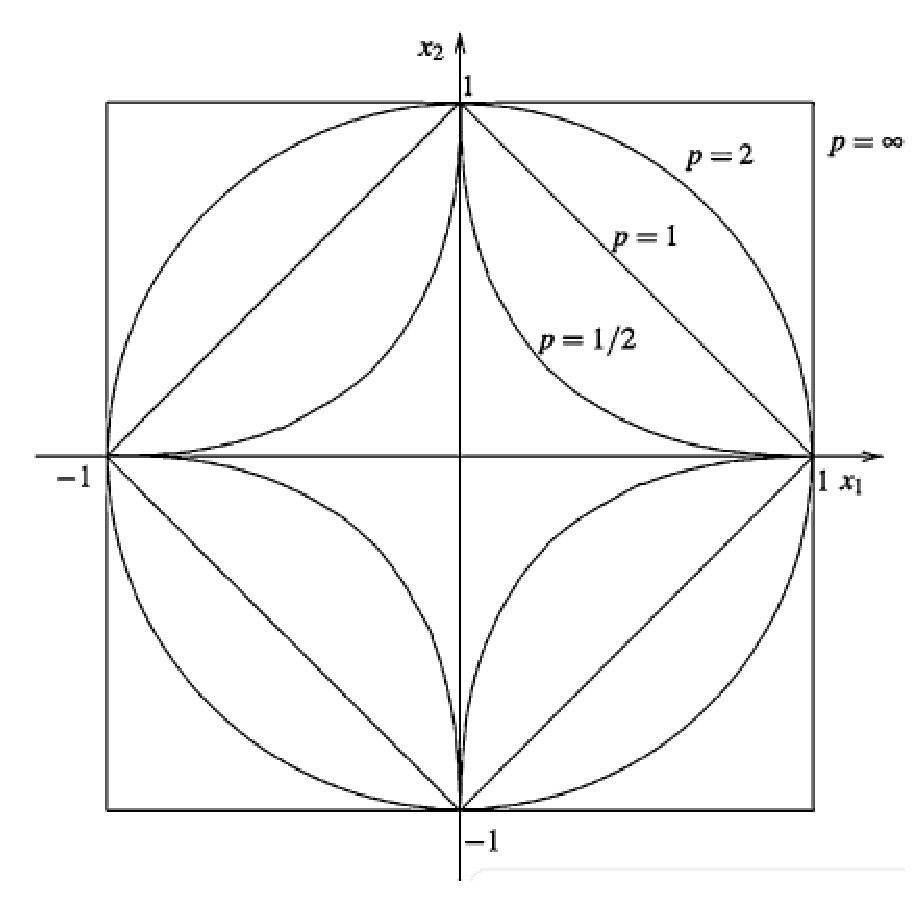
\includegraphics[scale=0.3]{Images/ch1/fig1.eps}
\caption{توپ واحد نُرم $l_{p}$ به ازای مقادیر مختلف $p$}
\label{fig1}
\end{figure}

اگر بجای استفاده از نُرم 
$\ell_{1}$
از نُرم
$\ell_{2}$
 استفاده کنیم، میزان خطا در بازیابی به شدت افزایش می‌یابد. با توجه به شکل
\ref{fig2}
علت این خطا کاملا مشهود است. همانگونه که از شکل مشخص است به ازای نُرم دوم پاسخ محاسبه شده لزوما تنک نیست که با فرض مسأله در تناقض است
\cite{boche2015compressed}.

\begin{figure}
\centering
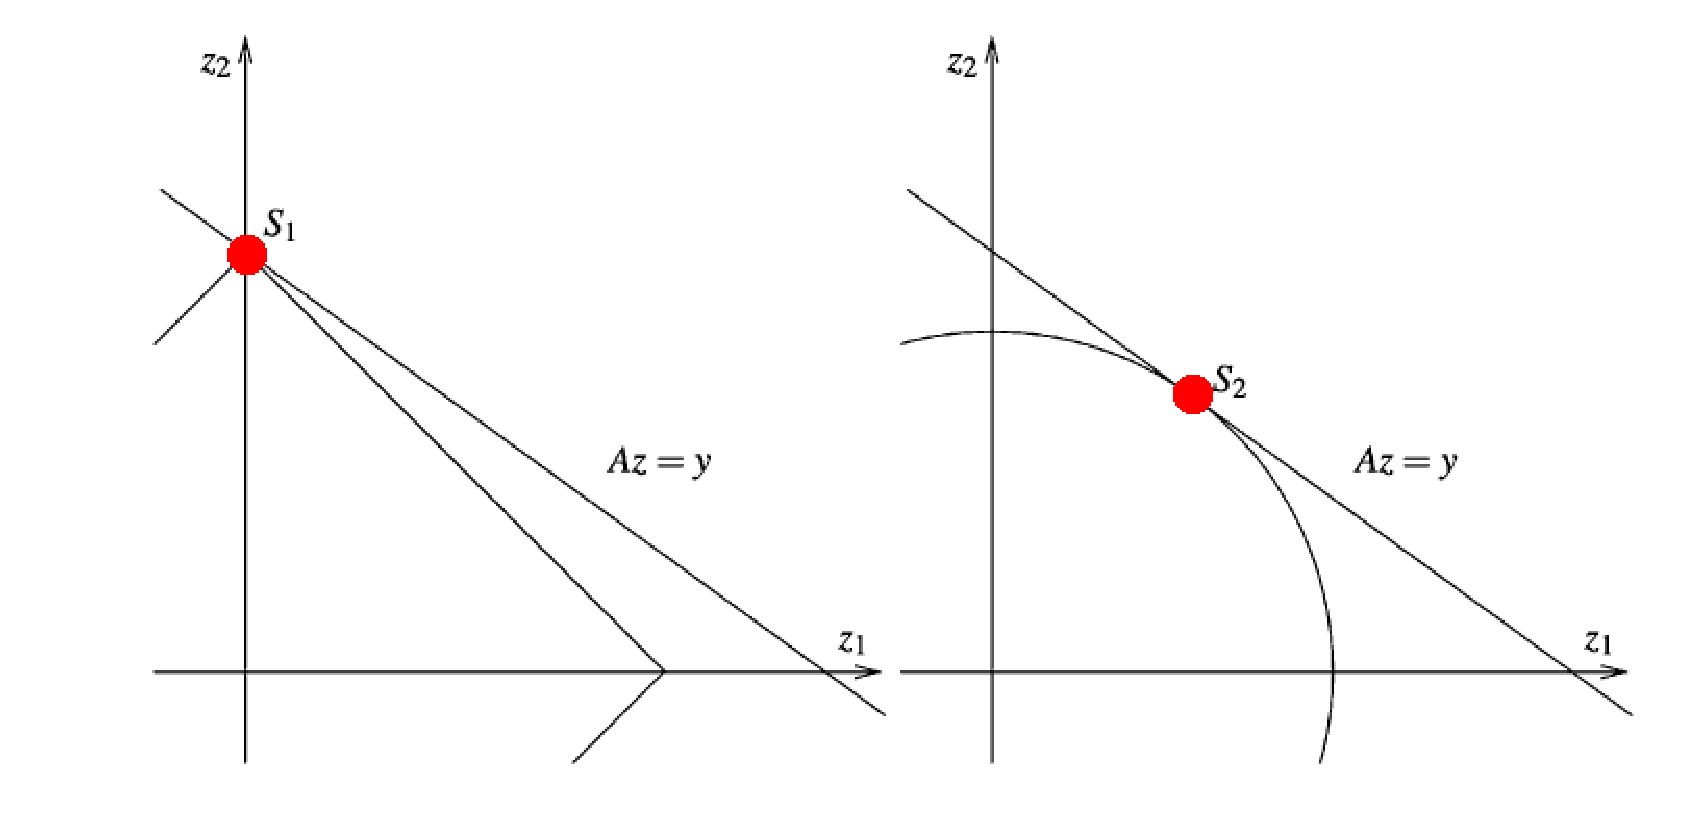
\includegraphics[scale=0.3]{Images/ch1/fig2.eps}
\caption{توپ واحد نُرم مراتب مختلف}
\label{fig2}
\end{figure}






 از روش‌های جایگزین جهت بازیابی سیگنال تنک می‌توان به روش‌های حریص
\LTRfootnote{Greedy}
همانند 
\lr{OMP}\LTRfootnote{Orthogonal Matching Pursuit}
و روش‌های مبتنی بر آستانه‌گذاری مثل 
\lr{IHT}\LTRfootnote{Iterative Hard Thresholding}
اشاره نمود. می‌توان نشان داد که با فرض مناسب، با استفاده از تمامی روش‌های فوق می‌توان سیگنال تنک را بازیابی نمود 
\cite{foucart2013mathematical}.


طراحی ماتریس نمونه‌برداری
$\bm{A}$
یک مساله‌ی جذاب در حسگری فشرده است و به عنوان یک مساله باز، بسیاری از محققان به دنبال تعیین یک ماتریس معین هستند که تمامی قید‌های حسگری فشرده را اقناع کند. برخی از ماتریس‌های معین برگرفته از تئوری تخمین تنک و کدینگ،‌ تا حد مناسبی شرایط بازیابی صحیح را برآورده می‌کنند ولی این ماتریس‌ها از باند بهینه تا حد قابل ملاحظه‌ای دور هستند. خوشبختانه با استفاده از ماتریس‌های تصادفی، شرایط مورد نیاز بازیابی صحیح برآورده می‌گردد. به عنوان دو مثال ساده، می‌توان به ماتریس تصادفی با درایه‌های نرمال و مستقل و یا ماتریس برنولی\LTRfootnote{Bernoulli}
اشاره نمود.
نتایج کلیدی در حسگری فشرده نشان می‌دهد که با احتمال بالا با استفاده از ماتریس تصادفی گوسی یا برنولی
$\bm{A}\in \R^{m \times N}$
، یک بردار 
$s$-تنک
$\bm{x}$
، با استفاده از نمونه‌برداری به صورت
$\bm{y}=\bm{A}\bm{x}$
با تعداد نمونه‌ی 
\begin{align}
\label{eq:eq4}
m \geq C s \log(N/s)
\end{align}
قابل بازیابی است. در عبارت فوق 
$C > 0$
یک مقدار حقیقی ثابت بوده و اثبات شده است که باند محاسبه شده بهینه است
\cite{foucart2013mathematical}.


با توجه به رابطه‌ی
\eqref{eq:eq4}
تعداد نمونه‌ی لازم جهت بازیابی یک سیگنال
$s$-تنک
با 
$s$
رابطه‌ی خطی دارد در صورتی که بعد سیگنال
$N$
، به صورت لگاریتمی با تعداد نمونه در ارتباط است. در صورتی که مقدار 
$s$
بسیار از مقدار
$N$
کوچکتر باشد، تعداد نمونه‌ها در مقایسه با بعد بردار مجهول کم می‌گردد و بازیابی سیگنال با استفاده از سیستم معادلات خطی فرومعین امکان‌پذیر خواهد بود
\cite{candes2006robust}. 


یکی دیگر از خصوصیات مهم در حسگری فشرده 
\textbf{پایداری}
است. به عبارت دیگر در زمانی که نمونه‌های دریافتی کمی غیر دقیق باشند و یا سیگنال مورد بررسی به صورت کامل تنک نباشد، خطای بازیابی  محدود و قابل کنترل است. در این شرایط با حل مساله‌ی کمینه‌سازی نُرم یک درجه‌ی دوم زیر، می‌توان پاسخ را پیدا نمود
\cite{foucart2013mathematical}.
\begin{align}
\label{eq:eq5}
\min \norm{\bm{z}}_{1} \quad \text{s.t.} \quad \norm{\bm{A}\bm{z}-\bm{y}}_{2} \leq \eta
\end{align}
در رابطه‌ی 
\eqref{eq:eq5}
،
$\eta$
برابر با توان نویز جمع‌شونده با سیگنال است.

بدون فرض پایداری، مساله‌ی حسگری فشرده قابل استفاده در کاربرد‌های عملیاتی نخواهد بود. زیرا در بسیاری از کاربرد‌ها، وجود نویز اجتناب‌ناپذیر است. در ادامه به بررسی مساله‌ی حسگری فشرده در حالت کوانتیزه
\LTRfootnote{Quantized}
می‌پردازیم.
%%%%%%%%%%%%%%%%%%%%%%%%%%%%
%%%%%%%%%%%%%%%%%%%%%%%%%%%%
%%%%%%%%%%%%%%%%%%%%%%%%%%%%
\section{حسگری فشرده‌ی کوانتیزه}
در سیستم‌های عملیاتی نمونه‌های دریافتی نمی‌توانند دقت بی‌نهایت داشته باشند و باید به یک الفبا با تعداد عناصر محدود نگاشته گردند.
در کاربرد های عملی هر نمونه (که ممکن است شامل بی نهایت هم باشد) به تعداد محدود و گسسته از مقادیر با دامنه‌ی محدود نگاشته گردد.  برای مثال اگر از یک سیستم کوانتایزر یکنواخت
\LTRfootnote{Uniform quantizer}
با 
$ B $
بیت در هر اندازه‌گیری استفاده کنیم، مقادیر به یکی 
$ 2^B $
مقدار گسسته نگاشته می‌شوند. باید توجه داشت که کوانتیزه کردن نمونه‌ها یک عمل برگشت‌ناپذیر است و همواره مقداری از اطلاعات در این فرآیند از بین می‌رود. 

مشوق اصلی در بررسی حسگری فشرده در حالت کوانتیزه، محدودیت‌های سخت‌افزاری در سیستم‌های دیجیتال است. 
در سیستم‌های سخت‌افزاری یکی از محدودیت‌های اساسی در  مبدل آنالوگ به دیجیتال
(\lr{ADC})
رخ می‌دهد. به عبارت دیگر مبدل آنالوگ به دیجیتال که وظیفه‌ی نمونه‌برداری و کوانتیزه کردن سیگنال ورودی را بر عهده دارد با محدودیت‌های زیر رو به رو است.
\begin{itemize}
\item{
\textbf{سرعت نمونه برداری:}
فرآیند کوانتیزاسیون حداکثر سرعت
\lr{ADC}
را به شدت محدود می‌کند. به طوری که اگر تعداد بیت‌های 
\lr{ADC}
به صورت خطی افزایش یابد، سرعت نمونه‌برداری به صورت نمایی کاهش می‌یابد.
}
\item{
\textbf{هزینه:}
با افزایش تعداد بیت در
\lr{ADC}
هزینه ساخت بالا می‌رود.
}
\item{
\textbf{اثرات غیرخطی}
با افزایش تعداد بیت ساخت قطعات الکترونیکی با اعوجاج کم سخت‌تر می‌شود.
}
\end{itemize}


با توجه به موارد ذکر شده در بالا اگر بتوان تعداد بیت‌های اندازه‌گیری را کاهش داد، به سخت‌افزار‌های بهتر و سریع تری دسترسی داریم
\cite{laska2012regime}.
یکی دیگر از محدودیت‌های عملی در سیستم‌های کاربردی نرخ انتقال داده است. در این سیستم‌ها معمولا چندین بخش مختلف نیاز به ارتباط با یکدیگر دارند که نرخ انتقال اطلاعات بین آنها محدود است. 

در ادامه اثر تعداد بیت و نرخ نمونه‌برداری در خطای بازیابی بررسی شده است.


\section{مدل حسگری فشرده کوانتیزه}
با فرض اینکه سیستم به صورت یکنواخت از سیگنال ورودی نمونه بردارد و تعداد بیت در هر نمونه ثابت فرض شود، می‌توان نرخ حاصل از نمونه‌برداری را به صورت 
$ \mathfrak{B}=mB $
بیان نمود.  
$ \mathfrak{B}$
در واقع نشان‌دهنده‌ی پهنای باند در اختیار جهت انتقال داده‌ها یا  بودجه بیت
\LTRfootnote{Bit budget}
است و در آن 
$m$
برابر با تعداد نمونه‌ها و 
$B$
تعداد بیت در هر نمونه است.
 مدل نمونه‌برداری خطی
\eqref{eq:eq1}
 با اضافه شدن قیود عملی به صورت 
\eqref{eq:eq6}
بیان می‌شود.
\begin{align}
\label{eq:eq6}
\bm{y}_{\mathcal{Q}} =A(\bm{x}):= \mathcal{Q}_{B}\left(\bm{A}(\bm{x}+\bm{n})+\bm{e}\right)
\end{align}
در عبارت فوق ‍
$\bm{n}$
و
$\bm{e}$
به ترتیب نویز قبل و بعد از نمونه‌برداری و
$\mathcal{Q}_{B}$
تابع کوانتایزر 
$B$
بیتی که مقادیر حقیقی نمونه‌های حسگری فشرده را به الفبای گسسته‌ی 
$\mathfrak{U}$
با 
$2^{B}$
عضو می‌نگارد. در این بخش بردار
$\bm{n}$
به صورت یک بردار تصادفی که هر درایه‌ی آن از توزیع نرمال با میانگین صفر و واریانس
$\sigma_{\bm{n}}^{2}$
 است، انتخاب شده است. همچنین مقدار
$\norm{\bm{e}}_{2}$
را برابر با صفر در نظر می‌گیریم.


با فرض 
$ \mathfrak{B}$
و نویز ثابت، کارایی سیستم را می‌توان بر اساس تعداد نمونه‌ها بررسی نمود. از طرف دیگر، با توجه به اینکه 
$B = \mathfrak{B}/m$
است،‌ می‌توانیم با کاهش تعداد نمونه‌ها، تعداد بیت در هر نمونه را افزایش دهیم که منجر به افزایش دقت در هر نمونه می‌گردد. بنابراین اگر ما تعداد نمونه‌ی کمتری برداریم، می‌توانیم به هر نمونه تعداد بیت بیشتری اختصاص دهیم ولی در اثر نویز ممکن است با اخذ هر نمونه تعداد بیت بیشتری حامل داده‌های غلط باشند.

در مرجع
\cite{laska2012regime}
با فرض نویز مستقل و گوسی تعداد بیت بهینه که متوسط مربع خطا
\LTRfootnote{MSE}
را کمینه می‌کند طبق رابطه‌ی 
\eqref{eq:eq7}
به دست آمده است.
\begin{align}
\label{eq:eq7}
B \approx \dfrac{1}{2}\log_{2}\left( \dfrac{\norm{\bm{x}}_{2}^{2}}{\sigma^{2}_{\bm{n}}}\dfrac{m}{N}\right)
\end{align}

با فرض نمونه‌برداری یکنواخت و
$ \mathfrak{B} $
ثابت معادله‌ی فوق را می توان به صورت زیر بازنویسی کرد.
\begin{align}
\label{eq:eq8}
\log_{2}\left( \dfrac{\norm{\bm{x}}_{2}^{2}}{N \sigma^{2}_{\bm{n}}}\right)\approx \dfrac{2\mathfrak{B}}{m}-\log_{2}\left(m\right)
\end{align}

عبارت سمت چپ بیانگر نسبت سیگنال به نویز
(\lr{SNR})
است. با توجه به 
\eqref{eq:eq7}
سیگنال را در دو حالت مختلف می‌توان بررسی کرد.
\begin{itemize}
\item{
\textbf{سیگنال‌های قوی:}
در این حالت سمت چپ عبارت عدد بیشتری دارد بنابراین برای حداقل شدن خطا باید تعداد اندازه گیری‌ها کم و تعداد بیت در هر اندازه‌گیری بالا باشد. 
}
\item{
\textbf{:سیگنال‌های ضعیف}
در این حالت بر خلاف حالت قبلی بهتر است از تعداد نمونه‌های بیشتر با تعداد بیت کمتر در هر نمونه استفاده شود.
}
\end{itemize}

\section{باند خطا}
در مرجع
\cite{laska2012regime}
یک باند خطا برای سیستم نمونه برداری شده به صورت زیر بدست آمده است.
\begin{theorem}
\label{thorem:thm1}
فرض کنید، 
$\bm{y}_{\mathcal{Q}} =A(\bm{x}):= \mathcal{Q}_{B}\left(\bm{A}(\bm{x}+\bm{n})\right)$
و سیگنال
$\bm{x}\in \R^N$
دارای  پشتیبان
$\Omega \in \lbrace 1,\cdots,N\rbrace$
با اندازه‌ی 
$|\Omega|=s$
باشد. درایه‌های 
$\Omega$
به صورت تصادفی با توزیع یکنواخت و دامنه‌ی عناصر غیر صفر به صورت 
$ x_{i} \in \Omega \sim \mathcal{N}\left( 0,\sigma_{\bm{x}}^{2} \right) $
بدست آمده‌اند. درایه‌های بردار نویز
$\bm{n}\in \R^m$ 
به صورت تصادفی از توزیع نرمال با میانگین صفر و واریانس
$\sigma^{2}_{\bm{n}}$
انتخاب شده است. همچنین فرض کنید که درایه‌های ماتریس نمونه‌برداری
$\bm{A}\subset \R^{m\times N}$
در شرط 
\lr{RIP}\LTRfootnote{Restricted Isometry Property}
از مرتبه‌ی
$s$
و ثابت
$\delta$
صدق کند. با انتخاب مناسب 
$\mathcal{Q}$
 و مقدار ثابت 
$\mathfrak{B}=mB$
، مقدار 
\lr{MSE}
در شرط زیر صدق خواهد کرد.
\begin{align}
\label{eq:eq9}
\mathbb{E}\left( \norm{\bm{x}-\hat{\bm{x}}}_{2}^{2} \right) \leq \dfrac{2s}{\mathfrak{B}\left( 1-\delta\right)} \left[ s\sigma^{2}_{\bm{x}}B2^{-2B}+N\sigma^{2}_{\bm{n}}B\left(1+2^{-2B}\right)\right]\\ \nonumber
\qquad \qquad+\dfrac{s}{\left( 1-\delta\right)}\left(\dfrac{\mathfrak{B}}{B}-1\right)\mathfrak{S}
\end{align}
که در آن 
$ \mathfrak{S}=\max_{i\neq j}\vert \mathbb{E}\mathcal{Q}_{B}\left(\bm{A}(\bm{x+n})\right)_{i}\mathcal{Q}_{B}\left(\bm{A}(\bm{x+n})\right)_{j}\vert $
است.
\end{theorem}
\begin{proof}
 این قضیه در 
\cite{laska2012regime}
اثبات شده است.
\end{proof}
در معادله مذکور عبارت 
$ s\sigma^{2}_{\bm{x}}B2^{-2B} $
بیانگر خطای ناشی از کوانتیزاسیون سیگنال و عبارت 
$ N\sigma^{2}_{\bm{n}}B\left(1+2^{-2B}\right) $
اثر نویز و کوانتیزاسیون را به صورت همزمان نشان می‌دهد. عبارت 
$ \left(\dfrac{\mathfrak{B}}{B}-1\right)\mathfrak{S} $
نشان دهنده‌ی اثر همبستگی در اندازه گیری کوانتیزه شده است.

در بسیاری از سناریو‌های حسگری فشرده، انتظار داریم که مقدار عبارت آخر در سمت راست رابطه‌ی 
\eqref{eq:eq9}
به صفر میل کند. برای مقادیر بزرگ 
$B$
، در مرجع 
\cite{gray1998quantization}
نشان داده شده است که این عبارت با تقریب خوبی به صفر میل می‌کند. بنابراین انتخاب مقدار بهینه‌ی 
$B$
با متعادل‌سازی دو عبارت داخل کروشه بستگی دارد. 

باند خطای محاسبه شده در رابطه‌ی 
\eqref{eq:eq9}
برای سیگنال‌های تنک کامل به دست آمده است. در صورتی که دسته‌ی مهم دیگری از سیگنال‌ها در پردازش سیگنال دیجیتال، سیگنال‌های فشرده‌پذیر هستند. در سیگنال‌های فشرده‌پذیر قسمت عمده‌ی توان در 
$s$
مولفه از سیگنال به ترتیب نزولی دامنه، قرار دارد. در این حالت 
$N-s$
مولفه‌ی دیگر را دنباله‌ی سیگنال می‌نامیم. برای چنین سیگنالی، دنباله‌ی سیگنال همانند نویز فرض می‌شود و در فرآیند بازیابی حذف می‌گردد
\cite{davenport2012pros,davies2011sample}.
نتایج قضیه‌ی
\ref{thorem:thm1}
را می‌توان به سیگنال‌های فشرده‌پذیر تعمیم داد. در این حالت مقادیر کوچک و غیر صفر به صورت نویز مدل می‌شوند.



برای مقایسه‌ی اثر توان سیگنال و تعداد بیت دو پارامتر 
\lr{ISNR}\LTRfootnote{Input SNR}
و
\lr{RSNR}\LTRfootnote{Reconstruction SNR}
را به صورت زیر تعریف می‌کنیم.
\begin{align}
\label{eq9}
ISNR := 10\log_{10}\left( \dfrac{\mathbb{E}\left( \norm{\bm{x}}_{2}^{2} \right)}{\mathbb{E}\left( \norm{\bm{n}}_{2}^{2} \right)} \right)
\end{align}
\begin{align}
\label{eq10}
RSNR := 10\log_{10}\left( \dfrac{\norm{\bm{x}}_{2}^{2}}{\norm{\bm{x}-\bm{x}^{\star}}_{2}^{2}} \right)
\end{align}

در شکل
\ref{fig3}
مقدار 
\lr{MSE}
به ازای 
\lr{ISNR}های
مختلف نشان داده شده است.
\begin{figure}[H]
\centering
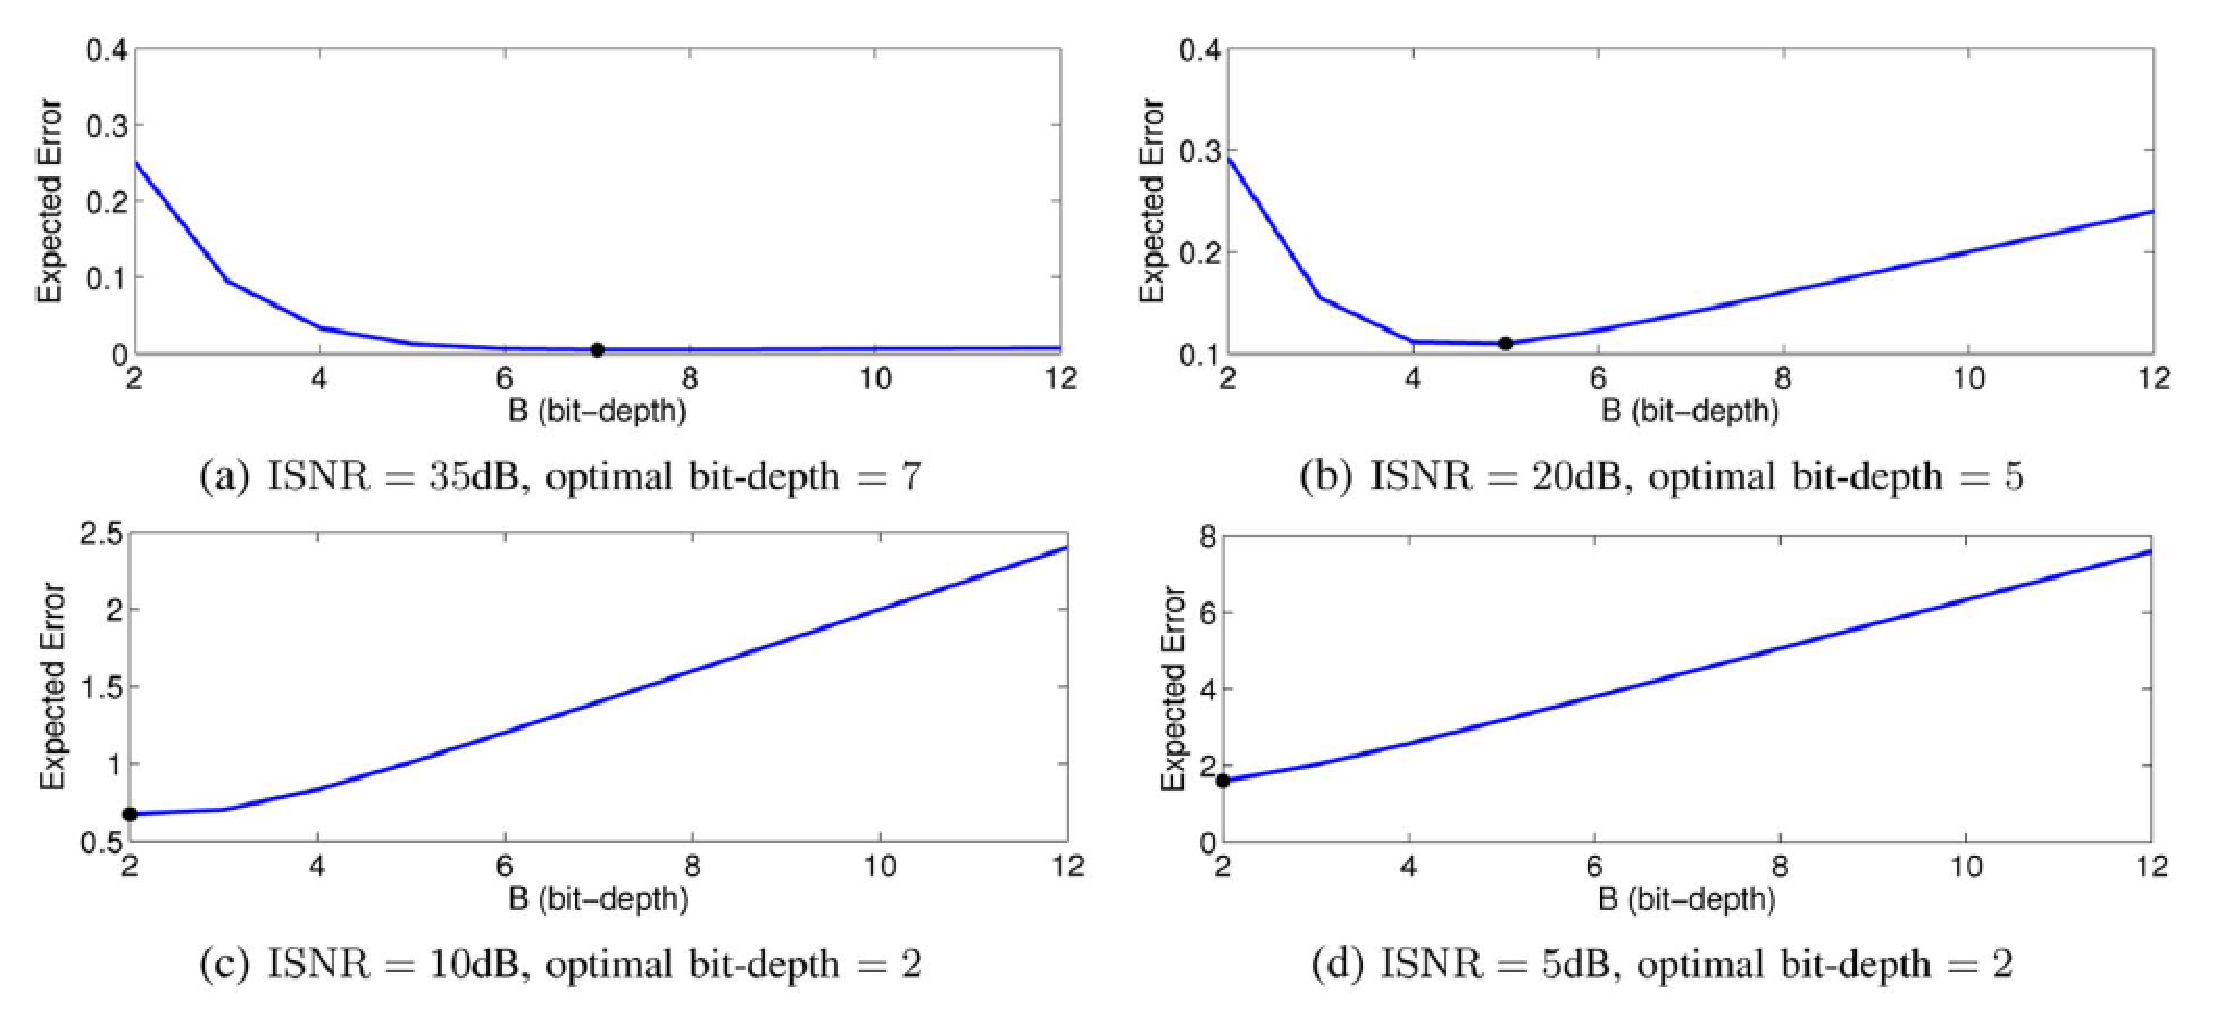
\includegraphics[scale=0.34]{Images/ch1/fig3.eps}
\caption{مقدار 
\lr{MSE}
به ازای 
\lr{ISNR}های
مختلف\cite{laska2012regime} }
\label{fig3}
\end{figure}

با توجه به شکل برای سیگنال‌های قوی تعداد بیت بیشتر و برای سیگنال‌های ضعیف تعداد بیت کمتر منجر به کاهش خطا می‌گردد.
نکته‌ی قابل توجه در این نمودار رفتار خطا به ازای افزایش تعداد بیت است. همان‌گونه که مشخص است در همه‌ی حالات تعداد بیت بالا لزوما بهینه نیست. علاوه بر این، همانگونه که انتظار داشتیم، حداقل خطای بازیابی به ازای 
\lr{ISNR}
پایین، در تعداد بیت کم رخ می‌دهد.

به عنوان یک نتیجه‌ی کلی می‌توان گفت که در صورتی که سیگنال مورد بررسی دارای نسبت سیگنال به نویز پایین باشد، با تعداد بیت کم نیز می‌توان سیگنال را بازیابی نمود.
\section{حسگری فشرده تک بیتی}
بررسی‌ها بر روی محدودیت تعداد بیت در هر نمونه نشان داد که تنها یک بیت در هر نمونه از سیگنال جهت بازیابی صحیح سیگنال کافی است
\cite{boufounos20081} .
در این حالت مدل نمونه‌برداری از بردار 
$\bm{x}$
به صورت رابطه‌ی 
\eqref{eq:eq10}
خواهد بود.
\begin{align}
\label{eq:eq10}
\bm{y}= \text{sign}\left(\bm{A}\bm{x}\right).
\end{align}


نمونه‌برداری تک بیتی در  مسایل آماری و مهندسی کاربرد دارد. از کاربرد‌های نمونه‌برداری تک بیتی ‌می‌توان به موارد زیر اشاره نمود.
\begin{itemize}
\item{
\textbf{
بازیابی سیگنال و مبدل‌های آنالوگ به دیجیتال.
}
وظیفه‌ی یک مبدل آنالوگ به دیجیتال نمونه‌برداری از سیگنال آنالوگ
$ \bm{x} $
و به دست آوردن تقریب دیجیتال
$ \widehat{\bm{x}}$
است. در صورتی که سیگنال تنک باشد، تعداد نمونه‌ها کاهش می‌یابد. در عمل تعداد بیت بالا در سخت‌افزار منجر به گران‌تر شدن سخت‌افزار می‌شود ولی نمونه‌برداری تک بیتی به معنای یک مقایسه کننده است که پیاده‌سازی آسان و ارزان دارد. 
}
\item{
\textbf{
رگرسیون دودویی.
}\LTRfootnote{Binary regression}
در یکی از مدل‌های رگرسیون منطقی، فرآیند تصمیم‌گیری یک فرد را با بردار
$ \bm{a}_{i} $
و پاسخ فرد در مورد یک موضوع را با بردار
$ \bm{x} $
نشان می‌دهند. اگر 
$ \langle \bm{a}_{i}  , \bm{x}\rangle > \nu_{i} $
باشد، پاسخ مثبت و در غیر این صورت پاسخ منفی است. در رگرسیون دودویی تنک همانند حسگری فشرده هدف پیدا کردن 
$ \bm{x} $
است. بنابراین از نتایج حسگری فشرده تک بیتی می‌توان در این حوزه نیز استفاده نمود.
}
\item{
\textbf{
الگوریتم‌های پخش عمومی.
}\LTRfootnote{Streaming algorithms and broadcasting }
فرض کنید گره‌ی مرکزی\LTRfootnote{Centeral node}
فایل 
$ \bm{x} $
را دارد (که به صورت تنک مدل شده است) و می‌خواهد به یک یا چند گره که هرکدام  دقت متفاوت دارند، ارسال کند. یک گزینه پخش عمومی بیت‌های
$ \text{sign}\left( \langle \bm{a}_{i}  , \bm{x}\rangle - \nu_{i}  \right) $
است. گره‌های مقصد با توجه به دقت و سایر مشخصات خود و کانال، تعداد بیت لازم جهت بازیابی صحیح را دریافت می‌کند.
}
\end{itemize}

از طرف دیگر در بعضی مواقع با توجه به محدودیت در پهنای باند، توان و یا هزینه‌ی عملیاتی سیستم، استفاده از نمونه‌های تک بیتی تنها گزینه‌ی موجود است. به عنوان مثال می‌توان به برخی از گیرنده‌های دیجیتال باند وسیع یا سیستم‌های انبوه آنتنی
\LTRfootnote{Massive MIMO}
اشاره نمود
\cite{Yin2010,risi2014massive,jacques2013robust, baraniuk2017exponential}.


با فرض نمونه‌برداری به صورت
\eqref{eq:eq10}
بردار
$\bm{y}$
هیچ اطلاعاتی از دامنه‌ی بردار
$\bm{x}$
ندارد و در این حالت ما امیدواریم که تنها بتوانیم جهت بردار 
$\bm{x}$
را تخمین بزنیم. خوشبختانه، اگر با تغییر در مدل نمونه‌برداری، بجای آستانه‌ی صفر از آستانه‌های تصادفی (به عنوان مثال 
$\tau_{i} \sim \mathcal{N}(0,1)$
) برای هر نمونه استفاده گردد، اطلاعات دامنه‌ی سیگنال حفظ می‌شود. در این حالت مدل نمونه‌برداری به صورت 
\eqref{eq:eq11}
تغییر خواهد کرد.
\begin{align}
\label{eq:eq11}
\bm{y}= \text{sign}\left(\bm{A}\bm{x}-\bm{\tau}\right).
\end{align}
در بخش‌های آتی تفاوت بین دو رابطه‌ی 
\eqref{eq:eq10}
و  
\eqref{eq:eq11}
از دیدگاه هندسی بررسی شده است.


بخش عمده‌ای از تحقیقات در حسگری فشرده صرف بازیابی سیگنال‌های تنک شده است. در صورتی که بسیاری از سیگنال‌های طبیعی بعد از یک تبدیل تنک می‌گردند. به عنوان مثال سیگنال‌های سینوسی در فضای فوریه تنک هستند و یا تصاویر پس از تبدیل ویولت
\LTRfootnote{Wavelet}
تنک می‌گردند. در صورتی که از یک تبدیل متعامد استفاده کنیم، نتایج حسگری فشرده به سادگی قابل تعمیم به این حوزه خواهد بود. از سوی دیگر، دسته‌ای از سیگنال‌ها که دیکشنری-تنک نامیده می‌شوند، در یک دیکشنری غیر متعامد تنک هستند. برای مثال  سیگنال‌های رادار در چارچوب گابور
\LTRfootnote{Gabor frame}
تنک هستند. مساله‌ی دیکشنری‌های افزونه
\LTRfootnote{Redundant dictionary}
ابتدا در مرجع 
\cite{Candes2011}
بررسی شد و در ادامه در
\cite{Baraniuk2017}
به حسگری فشرده تک بیتی گسترش داده شده است.

\section{کار‌های قبلی}
در این بخش، کارهای انجام شده در زمینه‌ی حسگری فشرده‌ی تک بیتی به صورت مختصر مرور شده است.
در حسگری فشرده سنتی، نمونه‌ها به صورت اعداد اسکالر فرض می‌شدند. نویسندگان
\cite{boufounos20081}
مدل نمونه‌برداری را تغییر دادند و فرض کردند که تنها علامت مشاهدات در دسترس است. بر همین مبنا، الگوریتم بازیابی سیگنال را طراحی کردند. در 
\cite{laska2012regime}،
اثر تعداد بیت در هر نمونه برای سیگنال‌های قوی و ضعیف بررسی گردید و  استفاده از تعداد بیت کم در حالتی که سیگنال ورودی دارای نسبت سیگنال به نویز پایین است را پیشنهاد داد. در این میان تعداد زیادی الگوریتم جدید طراحی گردید که به عنوان مثال می‌توان به 
\lr{Matching Sign Pursuit (MSP)}،
\lr{Restricted-Step Shrinkage (RSS)}
و
\lr{Binary Iterative Hard Thresholding (BIHT)}
اشاره نمود
\cite{boufounos2009greedy,laska2011trust,jacques2013robust}.


در  
\cite{jacques2013robust}،
یک باند بالا برای خطای بازیابی بر اساس درجه تنکی و تعداد نمونه‌ها محاسبه گردید. 	علاوه بر این، معیار 
\lr{B$\epsilon$SE}
را برای ماتریس اندازه‌گیری معرفی نمود. این معیار مشابه معیار 
\lr{RIP}
در حسگری فشرده سنتی است. 

در ادامه نویسندگان
\cite{plan2013one}
، مساله‌ی حسگری فشرده‌ی تک بیتی را از دیدگاه هندسی بررسی کردند و یک پاسخ بهینه برای مساله‌ی حسگری فشرده تک بیتی ارائه دادند. در ادامه در 
\cite{plan2013robust}
حالت نویزی مساله نیز بررسی گردید.

در 
\cite{knudson2016one}
دو الگوریتم جهت بازیابی کامل سیگنال (اندازه و جهت)‌ ارائه گردید.  الگوریتم اول از آستانه‌های تصادفی جهت بازیابی سیگنال استفاده می‌کند و در الگوریتم دوم اندازه و جهت سیگنال به صورت جداگانه به دست می‌آیند. در 
\cite{kamilov2012one}
یک الگوریتم وفقی با استفاده از 
\lr{GAMP\LTRfootnote{Generalized approximate message passing algorithm}}
طراحی گردید که در آن آستانه‌ها در طول زمان نمونه‌برداری به روز می‌گردند.

با این وجود، تحقیقات گسترده‌ای به همراه الگوریتم‌های مختلف جهت کاهش خطای بازیابی در حسگری فشرده‌ی تک بیتی طراحی گردید.  در  
\cite{Guentuerk2003}
، از کوانتایزر تک بیتی سیگما-دلتا جهت رسیدن به نرخ کاهش نمایی استفاده گردید. در  
\cite{baraniuk2017exponential}،
با استفاده از همین رویکرد، یک سناریوی نمونه‌برداری و بازیابی وفقی طراحی شده است که با استفاده از آن می‌توان به نرخ کاهش نمایی  در حسگری فشرده‌ی تک بیتی دسترسی پیدا نمود.

کار جدید بارانیوک
\LTRfootnote{Baraniuk}
و همکاران، نشان داد که با استفاده از الگوریتم مبتنی بر بهینه‌سازی محدب و یا آستانه‌گذاری می‌توان اندازه و جهت سیگنال‌های دیکشنری-تنک را بازیابی نمود
\cite{Baraniuk2017}.

در این پایان‌نامه، ما از آستانه‌گذاری وفقی برای بازیابی سیگنال‌های دیکشنری تنک استفاده نموده‌ایم و جهت اثبات مباحث هندسه‌ی ابعاد بالا بکار رفته است.

\section{نشانه‌گذاری}
در این قسمت، نشانه‌گذاری مورد استفاده در پایان‌نامه بیان شده است.
بردار‌ها و ماتریس‌ها به ترتیب با حروف کوچک و بزرگ توپر نشان داده شده است. 
 $ \bm{v}^T $ 
 و
 $ \bm{v}^{\ast} $
به ترتیب نشان‌دهنده‌ی عملیات انتقال و مزدوج-انتقال بردار 
$ \bm{v} $
است. مقادیر مثبت، صحیح و ثابت با حروف بزرگ و کوچک لاتین نشان داده شده است که ممکن است خط به خط تغییر کند.
مقدار نُرم 
$\ell_2$ 
بردار
$ \bm{v} \in \R^n $
به صورت
$ \norm{\bm{v}}_2= \sqrt{\Sigma_i v_i^2} $
و نُرم 
$\ell_1$ 
به صورت
 $ \norm{\bm{v}}_1= \Sigma_i |v_i|$
و نُرم
$ \ell_{\infty} $
به صورت
$ \norm{\bm{v}}_{\infty}= \max_{i} |v_{i}| $
 تعریف می‌گردد.
  $ \norm{\bm{v}}_0 $
 نشان‌دهنده‌ی تعداد عناصر غیر صفر بردار
 $ \bm{v} $
 است و اگر
 $ \norm{\bm{v}}_0 \leq s$
 باشد،  بردار را
$s$-تنک
می‌نامیم. 
$ B_1^n := \{\bm{v}\in \R^n : \norm{\bm{v}}_{1}\leq 1 \} $ 
برابر با توپ $ \ell_1 $، 
$ B_2^n := \{\bm{v}\in \R^n : \norm{\bm{v}}_{2}\leq 1 \} $
برابر با توپ $ \ell_2 $ و 
$ S^{n-1}:= \{\bm{v}\in \R^n : \norm{\bm{v}}_{2}= 1 \} $
نشانگر کره واحد اقلیدسی است.
در طول این پایان‌نامه،
 $ d_{G}\left(\bm{v},\bm{u}\right):=1/\pi \arccos\langle \bm{v},\bm{u} \rangle $
نشانگر فاصله‌ی نرمالیزه‌ی ژئودزیک
\LTRfootnote{Normalized geodesic distance}
بین دو بردار 
$ \bm{u} $
و
$ \bm{v}$
روی 
$ S^{n-1} $ 
است. 

\section{طرح کلی}

در فصل
\ref{ch:HDE}
رویکرد هندسی در حوزه‌ی آشکارسازی و ابزارها به همراه مثال ارائه گردیده است. در ادامه مدل بیان شده به حسگری فشرده تعمیم یافته است.
پس از بیان مقدمات و ابزار‌های مورد نیاز جهت تحلیل موضوع به صورت هندسی، در ابتدای فصل
\ref{ch:main}
مساله‌ی سیگنال‌های دیکشنری تنک بررسی شده است. در این بخش ابتدا اهمیت سیگنال‌های دیکشنری تنک بیان گردیده و در ادامه به بیان چارچوب ریاضی آن پرداخته‌ایم.
در ادامه با بیان مدل سیستم مورد بررسی و همچنین تعاریف مورد نیاز الگوریتم پیشنهادی جهت بازیابی سیگنال دیکشنری تنک با استفاده از نمونه‌های تک بیتی ارائه شده و سپس، تحلیل تئوری و ضمانت‌های ریاضی الگوریتم بیان گردیده است.

در انتها، در فصل آخر، تنایج شبیه‌سازی الگوریتم پیشنهادی به همراه مقایسه با الگوریتم موجود، آورده شده است.

اثبات ریاضی نتایج در پیوست آورده شده است.




\chapter{تخمین در ابعاد بالا با رویکرد هندسی}
\label{ch:HDE}
\newpage
\section{مقدمه}
در این بخش یک چارچوب هندسی جهت حل مساله‌ی تخمین در ابعاد بالا بیان گردیده است. همچنین با ارایه‌ی تصویر شهودی از هندسه ابعاد بالا، نتایج هندسه‌ی محدب مجانبی
\LTRfootnote{asymptotic convex geometry}
 مساله‌ی تخمین و نتایج هندسی مقایسه شده است. نظریه‌های مطرح شده با کاربرد در بازیابی تنک، تکمیل ماتریس، کوانتیزه کردن، رگرسیون خطی و منطقی و مدل خطی عمومی، توضیح داده شده است. 
\subsection{تخمین مقید}
در این بخش،  چهارچوب ریاضی مساله‌ی تخمین با استفاده از قیود در ابعاد بالا بیان گردیده است. در این مساله، هدف تخمین نقطه‌ی 
$\bm{x}$
با استفاده از تعداد کمی نمونه‌ی مستقل به صورت 
$y_1,\cdots,y_m$
است که در یک مجموعه‌ی شدنی مشخص
$\mathcal{K} \subseteq \R^{n}$
قرار می‌گیرد. نقطه‌ی 
$\bm{x}$
می‌تواند نشان‌دهنده‌ی یک سیگنال در پردازش سیگنال، یک پارامتر از توزیع در آمار و یا یک ماتریس نامشخص در تکمیل ماتریس باشد. مجموعه‌ی شدنی
$\mathcal{K} $
دارای خصوصیاتی است که انتظار می‌رود سیگنال
$\bm{x}$
داشته باشد و یا ما بر آن سیگنال تحمیل می‌کنیم.


هندسه‌ی ابعاد بالای مجموعه‌ی شدنی
\LTRfootnote{feasible set}
$\mathcal{K} $
، کلید درک مساله‌ی تخمین است. یک شهود قدرتمند در رابطه با شکل مجموعه‌ها در ابعاد بالا در حوزه‌ای که با نام هندسه‌ی محدب مجانبی شناخته می‌شود، ارائه شده است
\cite{ball1997elementary,brazitikos2014geometry}.
شهود ارائه شده منجربه  نتایج بسیار دقیقی شده که برخی از آن‌ها قابل استفاده در مساله‌ی تخمین هستند. هدف اصلی از این بخش در سه موضوع زیر خلاصه می‌گردد.
\begin{itemize}
\item{
ارائه‌ی یک شهود از هندسه‌ی ابعاد بالا‌ی مجموعه
}
\item{
بیان نتایج هندسه‌ی محدب مجانبی و تایید شهود ارائه شده
}
\item{
ایجاد پیوند بین مساله‌ی تخمین در ابعاد بالا و هندسه‌ی ابعاد بالا
}
\end{itemize}

قبل از ارائه نتایج اصلی در این قسمت چند مثال کاربردی از تخمین بیان شده است.  یک کلاس ویژه از مسایل تخمین مقید در حوزه‌ی حسگری فشرده طبقه‌بندی می‌گردند. در این دسته از مسایل 
$\mathcal{K}$
دارای خاصیت تنکی  و  در برخی موارد تنکی ساختار یافته است که در آن تنها برخی مقادیر مجاز به غیر صفر شدن هستند
\cite{rao2011tight}.


یک مثال دیگر از مساله‌ی تخمین مقید، مساله‌ی تکمیل ماتریس است
\cite{recht2010guaranteed,candes2010power}.
در این مساله، 
$\mathcal{K}$
شامل ماتریس‌های رتبه پایین است و نمونه‌ها درایه‌های ماتریس هستند.

در حالت کلی، لزومی مبنی بر خطی بودن مشاهدات نیست. به عنوان یک مثال خوب می‌توان به حسگری فشرده‌ی تک بیتی اشاره نمود که در آن از یک مدل غیر خطی استفاده شده است. به صورت عمومی می‌توان مدل 
$\mathbb{E} y_{i} = \theta (\langle\bm{a}_{i}, \bm{x}\rangle)$
را برای نمونه برداری در نظر گرفت
\cite{ai2014one,plan2013robust}.

در علم آمار، این کلاس از مساله‌ی تخمین را می‌توان به صورت رگرسیون خطی (برای مشاهدات همراه با نویز)، رگرسیون منطقی (برای مشاهدات باینری) و مدل عمومی (برای مشاهدات غیر خطی)،  تفسیر نمود.

تمامی مثال‌های بیان شده در ادامه به صورت دقیق بررسی شده است. با این حال، هدف اصلی از این بخش، ارائه‌ی یک مدل فراگیر جهت استفاده در یک مجموعه‌‌ی شدنی عمومی است.

\section{مساله‌ی تخمین در ابعاد بالا}
فرض کنید که می‌خواهیم سیگنال مجهول 
$\bm{x}$
را تخمین بزنیم. فرض می‌کنیم که نمونه‌برداری به صورت تصادفی و مستقل  با استفاده از یک توزیع وابسته به 
$\bm{x}$
به صورت زیر اخذ شده است.
\begin{align}
\label{eq:eq12}
y_{i} \sim \text{distribution} (\bm{x}), \quad i= 1,\cdots,m 
\end{align}

بنابراین ما در پی بازیابی سیگنال 
$\bm{x}\in \R^{n}$
از بردار مشاهدات 
$\bm{y}\in \R^{m}$
هستیم. 
\subsection{ساختار‌های با پیچیدگی پایین}
در بسیاری از مواقع ما یک سری ویژگی برای بردار 
$\bm{x}$
در نظر می‌گیریم و یا حتی در برخی از مواقع بر آن تحمیل می‌کنیم.  می‌توان اطلاعات اضافه را به صورت زیر فرمول‌بندی نمود.
\begin{align*}
\bm{x} \in \mathcal{K}
\end{align*}
که در آن 
$\mathcal{K}$
یک مجموعه‌ی ثابت و زیرمجموعه‌ی 
$\R^{n}$
است که آن را مجموعه‌ی شدنی می‌نامیم. این  یک فرض بسیار عمومی و انعطاف‌پذیر است. در این مرحله هیچ خاصیت ویژه‌ای برای 
$\mathcal{K}$
در نظر نمی‌گیریم. به عنوان مثال می‌توان مجموعه‌ی 
$\mathcal{K}$
را تنک فرض نمود. 

شکل 
\ref{fig4}
\cite{Plan2016}
مساله‌ی تخمین را توصیف می‌کند. نمونه‌برداری می‌تواند به صورت یک نگاشت از 
$\bm{x} \in \mathcal{K}$
به 
$\bm{y} \in \R^{n}$
فرض شود و تخمین یک نگاشت از 
$\bm{y} \in \R^{n}$
به 
$\hat{\bm{x}} \in \mathcal{K}$
است که در حالت ایده‌آل معکوس نگاشت نمونه‌برداری است.

\begin{figure}
\centering
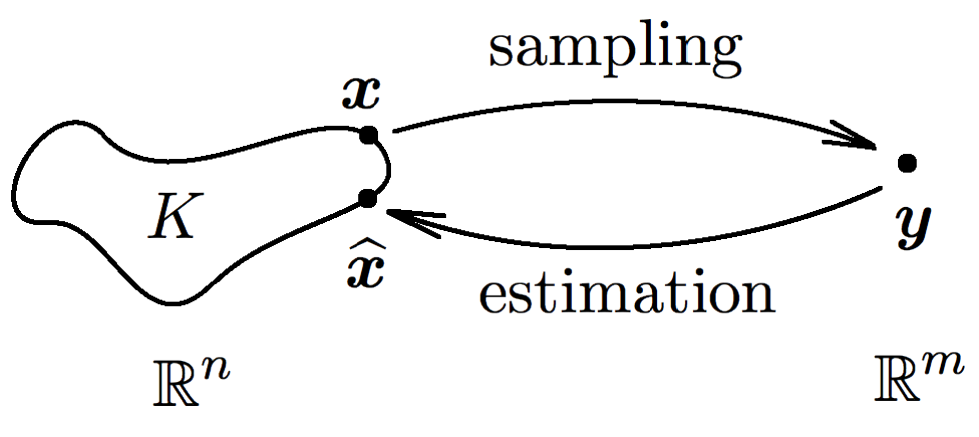
\includegraphics[scale=0.25]{Images/ch2/fig4.png}
\caption{توصیف گرافیکی مساله‌ی نمونه‌برداری و تخمین \cite{Plan2016}}
\label{fig4}
\end{figure}

اولین سوالی که به ذهن خطور می‌کند این است که اطلاعات و فرضیات موجود در مجموعه‌ی
$\mathcal{K}$
در ابعاد بالا چه کمکی به حل مساله می‌کند؟ جهت روشن شدن پاسخ مثال زیر را در نظر بگیرید. بردار 
$\bm{x}$،
$n$
بعد و بردار 
$\bm{y}$،
$m$
بعد دارد. قاعدتا، تخمین بردار 
$\bm{x}$
از
$\bm{y}$
با استفاده از 
\begin{align*}
m = O\left( n \right)
\end{align*}
مشاهده امکان‌پذیر است. حال فرض کنید که محدودیت 
$\bm{x} \in \mathcal{K}$
اضافه گردد. اگر 
$\mathcal{K}$
دارای بعد جبری
$\text{dim}(\mathcal{K})=d$
پایین باشد
$d \ll n$
، در این صورت 
$\bm{x}$
،
$d$
درجه‌ی آزادی خواهد داشت. بنابراین در این حالت تخمین با استفاده از نمونه‌های کمتر نیز امکان‌پذیر خواهد بود.
\begin{align*}
m = O\left( d \right)=o\left( n \right)
\end{align*}

این موضوع که مجموعه‌ی شدنی دارای بعد جبری کوچک باشد، به ندرت اتفاق می‌افتد. برای مثال، مجموعه‌ی تمام بردار‌های 
$s$-تنک
در 
$\R^{n}$
دارای بعد 
$n$
است. با این وجود، شهود در رابطه با بعد-پایین معتبر است. مجموعه‌های شدنی طبیعی، همانند تصاویر و ماتریس مجاورت شبکه، به نظر می‌رسد که دارای بعد پایین باشند. مجموعه‌ی
$\mathcal{K}$
ممکن است که دارای بعد بالا باشد ولی در حقیقت 
\textbf{بعد موثر}\LTRfootnote{Effective dimenstion}
آن پایین است. در ادامه‌ی این بخش،‌ با استفاده از این شهود موارد زیر بررسی شده است.
\begin{itemize}
\item{
تعیین کمیت پیچیدگی برای زیرمجموعه‌های 
$\mathcal{K}$
در 
$\R^{n}$
}
\item{
ثابت کردن امکان تخمین با استفاده از نمونه‌های کمتر از بعد جبری 
$\mathcal{K}$
}
\item{
طراحی تخمین‌گر جهت بازیابی سیگنال
}
\end{itemize}

در بخش بعدی شکل مجموعه‌ی 
$\mathcal{K}$
در ابعاد بالا ، با استفاده از ابزار‌های هندسه‌ی محدب مجانبی بررسی شده است.

\section{مقدمه‌ای بر هندسه‌ی محدب ابعاد بالا}
هندسه‌ی محدب ابعاد بالا، شکل اجسام
\LTRfootnote{Bodies}
 محدب را برای مقادیر زیاد 
$n$
بررسی می‌کند. اجسام محدب، مجموعه‌های محدب بسته، کراندار و توپر هستند. این حوزه از ریاضی، برخی اوقات هندسه‌ی محدب مجانبی و آنالیز تابعی هندسی
\LTRfootnote{Geometric functional analysis}
نیز نامیده می‌شود
\cite{ball1997elementary,brazitikos2014geometry,pisier1999volume}.


سوال اصلی در هندسه‌ی محدب ابعاد بالا این است که 
\textit{جسم محدب به چه شکل است؟}
به عنوان یک پاسخ اولیه می‌توان گفت که جسم محدب
$\mathcal{K}$
دارای یک تنه
\LTRfootnote{Bulk}
و تعدادی شاخک 
\LTRfootnote{Outlier}
است. بخش عمده‌ی حجم 
$\mathcal{K}$
در داخل تنه قرار دارد ولی معمولا قطر آن کم است. از طرف دیگر شاخک‌ها حجم کمی دارند ولی در هنگام محاسبه‌ی قطر، مقدار زیادی را به خود اختصاص می‌دهند.

با مقیاس نمودن 
$\mathcal{K}$
، تنه معمولا به شکل یک توپ اقلیدسی و شاخک‌ها به صورت نازک و بلند از توده به سمت خارج کشیده شده است. شکل
\ref{fig5}
نمایش هایپربولیک برای اجسام ابعاد بالا را نشان می‌دهد.
\begin{figure}
\centering
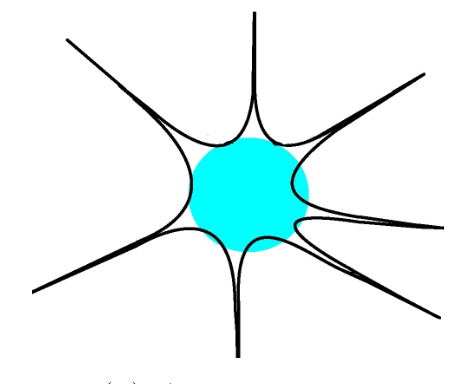
\includegraphics[scale=0.3]{Images/ch2/fig5.png}
\caption{نمایش هایپربولیک مجموعه‌های محدب ابعاد بالا\cite{Plan2016}}
\label{fig5}
\end{figure}

نمایش نشان داده شده در شکل
\ref{fig5}
محدب به نظر نمی‌رسد ولی به خوبی خواص ذکر شده را به تصویر می‌کشد. به عنوان مثال توپ نُرم 
$\ell_1$
را در نظر بگیرید. در این حالت مجموعه‌ی 
$\mathcal{K}$
به صورت زیر تعریف می‌گردد.
\begin{align*}
\mathcal{K}= B^{n}_{1}=\lbrace\bm{x} \in \R^{n}: \norm{\bm{x}}_{1}\leq 1 \rbrace
\end{align*}
در این حالت توپ اقلیدسی محاط در 
$\mathcal{K}$
را با 
$B$
نشان می‌دهیم. این توپ دارای قطر 
$2/\sqrt{n}$
است. می‌توان نشان داد که حجم
$B$
و 
$\mathcal{K}$
به صورت زیر قابل مقایسه هستند.
\begin{align*}
\text{vol}_{n} \left( B \right)^{1/n}\asymp \text{vol}_{n} \left( \mathcal{K} \right)^{1/n} \asymp \dfrac{1}{n}
\end{align*}
بنابراین، 
$B$
تشکیل دهنده‌ی تنه‌ی
$\mathcal{K}$
است و به صورت تقریبی بیشتر حجم 
$\mathcal{K}$
را تشکیل می‌دهد(شکل
\ref{fig6}). 

\begin{figure}
\centering
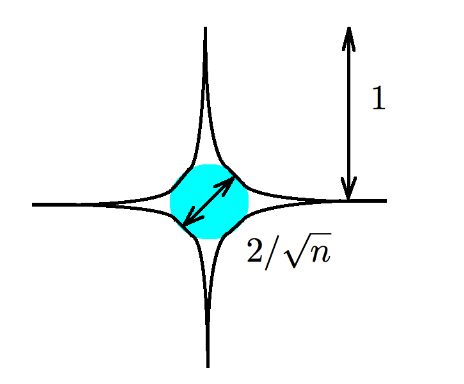
\includegraphics[scale=0.35]{Images/ch2/fig6.png}
\caption{نمایش ابعاد بالا‌ی توپ 
$l_{1}$
\cite{Plan2016}}
\label{fig6}
\end{figure}


\subsection{تمرکز حجم}
در این قسمت تحلیل ریاضی تایید‌کننده‌ی شهود مطرح شده در قسمت قبلی تحت عنوان تمرکز حجم 
\LTRfootnote{Concentration of volume}
بیان شده است.  فرض کنید که مجموعه‌ی
$\mathcal{K}$
ایزوتروپیک باشد. یعنی برای یک بردار تصادفی انتخاب شده از 
$\mathcal{K}$
با توزیع یکنواخت، میانگین برابر صفر و ماتریس کوواریانس همانی باشد. به عبارت ریاضی
\begin{align*}
\mathbb{E}~ \bm{x} = 0 , \quad \mathbb{E} ~\bm{x}\bm{x}^{T} = \bm{I}_{n}.
\end{align*}
با محاسبه‌ی رد ماتریس در دو طرف معادله‌ی دوم در رابطه‌ی فوق داریم:
\begin{align*}
\mathbb{E}~ \norm{\bm{x}}_2^2 = n
\end{align*}
در این حالت حداقل
$90$
 درصد از حجم 
$\mathcal{K}$
 در یک توپ اقلیدسی با اندازه‌ی 
 $O(\sqrt{n})$
 قرار دارد.
 تمرکز حجم در ابعاد بالا به صورت قضیه‌ی زیر خلاصه می‌گردد.
\begin{theorem}
\label{theorem:thm2}
\cite[قضیه~3.2]{vershynin2015estimation}
فرض کنید
$\mathcal{K}$
یک جسم ایزوتروپیک در
$\R^{n}$
 و 
$\bm{x}$
یک بردار تصادفی باشد که با توزیع یکنواخت از 
$\mathcal{K}$
انتخاب شده است. برای بردار 
$\bm{x}$
داریم:
\begin{itemize}
\item{
(تمرکز حجم)
به ازای یک $t>1$ 
\begin{align}
\mathbb{P}\lbrace\norm{\bm{x}}_{2}>t\sqrt{n} \rbrace \leq \exp\left( -ct\sqrt{n}\right)
\end{align}
}
\item{
(پوسته‌ی نازک)
برای هر 
$\epsilon \in (0,1)$
یکی 
\begin{align}
\mathbb{P}\lbrace\vert \norm{\bm{x}}_{2}-\sqrt{n}\vert > \epsilon\sqrt{n} \rbrace \leq C \exp\left( -c\epsilon^{3}\sqrt{n}\right)
\end{align}
}
\end{itemize}
\end{theorem}
\begin{proof}
 قضیه‌ی فوق در 
\cite{paouris2006concentration}
اثبات شده است.
\end{proof}

تعبیر هندسی تنه و شاخک به ما کمک می‌کند که بتوانیم یک برش تصادفی از 
$\mathcal{K}$
را تصور کنیم. فرض کنید که 
$E$
یک زیرفضای تصادفی از
$\R^{n}$
با بعد ثابت
$d$
باشد. در این حالت اگر
$d$
به اندازه‌ی کافی کوچک باشد، انتظار داریم که 
$E$
از تنه‌ی
$\mathcal{K}$
عبور کند و با شاخک‌ها برخورد نداشته باشد. به این ترتیب 
$\mathcal{K}\cap E$
خود یک توپ خواهد بود (شکل
\ref{fig7}).
قضیه‌ی دیورتزکی
\LTRfootnote{Dvoretzky}
این موضوع را به صورت ریاضی بیان می‌کند.
\begin{figure}
\centering
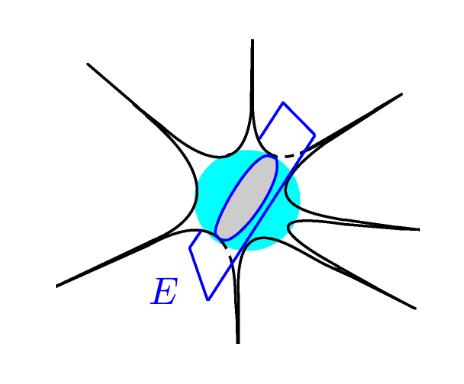
\includegraphics[scale=0.35]{Images/ch2/fig7.png}
\caption{نمایش ابعاد بالا‌ی  
$\mathcal{K}\cap E$
\cite{Plan2016}}
\label{fig7}
\end{figure}

\begin{theorem}
\label{theorem:thm3}
\cite[قضیه~3.3]{vershynin2015estimation}
فرض کنید 
$\mathcal{K}$
یک مجموعه‌ی محدب متقارن نسبت به مبدا، در 
$\R^n$
باشد. در این صورت بیضی محاط در 
$\mathcal{K}$
که بیشترین حجم را دارد توپ واحد اقلیدسی است. با فرض مقدار ثابت
$\epsilon \in (0,1)$
و انتخاب 
$d = c \epsilon^{-2} \log n$
بعد به صورت تصادفی از توزیع گرسمنین
\LTRfootnote{Grassmanian}
به عنوان زیرفضای
$E$
،یک 
$R\geq 0$
وجود دارد که با احتمال بالا (بیش از ۹۹ درصد)، رابطه‌ی زیر برقرار است.
\begin{align}
\left(1-\epsilon \right)RB^2_n \subseteq \mathcal{K}\cap E \subseteq \left(1+\epsilon \right)RB^2_n 
\end{align}
\end{theorem}
\begin{proof}
اثبات این قضیه در 
\cite{brazitikos2014geometry}
آورده شده است.
\end{proof}

بر خلاف تعبیر مشخص تقاطع یک جسم محدب با یک زیرفضای تصادفی با ابعاد پایین،‌ در حالتی که زیر فضای مورد نظر دارای بعد بالا باشد، نمی‌توان به سادگی شهود مشخصی برای تقاطع ارائه نمود. با این وجود می‌توان قطر این تقاطع را محاسبه نمود. یک کران برای این قطر تحت عنوان کران
$M^{\ast}$ 
ارائه شده است. قبل از بیان قضیه چند تعریف مقدماتی نیاز است که در ادامه بیان شده است.

\subsection{عرض میانگین}
با استفاده از عرض میانگین
\LTRfootnote{Mean width}
می‌توان مشخصات هندسی مهم یک مجموعه در 
$\R^n$
را به دست آورد. 
یک زیرمجموعه‌ی محدود 
$\mathcal{K}$
از 
$\R^n$
را فرض کنید ( محدب بودن، بسته و توپر بودن لازم نیست). عرض 
$\mathcal{K}$
در جهت مشخص
$\hat{\bm{n}}\in S^{n-1}$
به صورت کمترین فاصله‌ی بین دو ابرصفحه با بردار نرمال
$\bm{n}$
که شامل 
$\mathcal{K}$
است، تعریف می‌گردد. به عنوان مثال در شکل
\ref{fig8}
فاصله در جهت
$\hat{\bm{n}}$
برابر با 
$d$
است. به صورت تحلیلی، عرض در جهت 
$\bm{x}$
به صورت زیر تعریف می‌گردد.
\begin{align}
	\sup_{\bm{u},\bm{v}\in \mathcal{K}} \langle \hat{\bm{n}}, \bm{u}-\bm{v}  \rangle
\end{align}

\begin{figure}
\centering
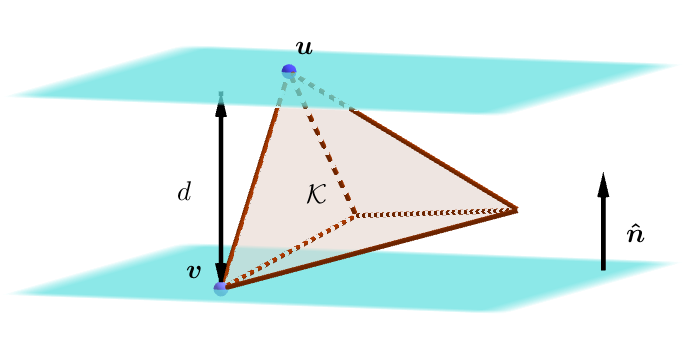
\includegraphics[scale=0.35]{Images/ch2/fig8.png}
\caption{عرض   
$\mathcal{K}$
در جهت
$\hat{\bm{n}}$
}
\label{fig8}
\end{figure}


اگر 
$\hat{\bm{n}}$
به صورت تصادفی با توزیع یکنواخت از 
$S^{n-1}$
انتخاب گردد، آنگاه عرض میانگین کروی
\LTRfootnote{spherical mean width}
مجموعه‌ی
$\mathcal{K}$
به صورت زیر تعریف می‌گردد.
\begin{align} 
\label{eq:eq13}
\tilde{w}\left(\mathcal{K}\right) := \mathbb{E} \sup_{\bm{u},\bm{v}\in \mathcal{K}} \langle \hat{\bm{n}}, \bm{u}-\bm{v}  \rangle
\end{align} 

در حوزه‌های دیگر همچون احتمال ابعاد بالا و تئوری یادگیری آماری، بسیار مرسوم است که بردار تصادفی با توزیع کروی
$\hat{\bm{n}} \sim \text{Unif}(S^{n-1})$
با یک بردار تصادفی نرمال استاندارد 
$\bm{g} \sim N (0,I_n)$
جایگزین گردد. برتری بردار
$\bm{g}$
نسبت به بردار
$\hat{\bm{n}}$
، درایه‌های مستقل آن است. عرض میانگین گوسی به صورت زیر تعریف می‌گردد.
\begin{definition}[عرض میانگین گوسی]
فرض کنید که 
$\bm{g} \sim N (0,I_n)$
بردار تصادفی نرمال استاندارد در
$\R^{n}$
باشد. در این صورت عرض میانگین گوسی یک مجموعه‌ی کراندار
$\mathcal{K}$
در 
$\R^{n}$
به صورت زیر تعریف می‌گردد.
\begin{align}
\label{eq:eq14}
w\left(\mathcal{K}\right) := \mathbb{E} \sup_{\bm{u},\bm{v}\in \mathcal{K}} \langle \bm{g}, \bm{u}-\bm{v}  \rangle
\end{align}	
\end{definition}
جهت خلاصه‌نویسی از این به بعد بجای عرض میانگین گوسی، از عبارت عرض گوسی استفاده می‌کنیم.


در نگاه اول مشخص است که عرض گوسی با ضریب 
$\sqrt{n}$
از عرض کروی بزرگتر است. با فرض
$\hat{\bm{n}}$
به صورت
$\hat{\bm{n}}= \bm{g} / \norm{\bm{g}}_{2}$
، می‌توان عرض  کروی را به صورت زیر بازنویسی نمود. 
\begin{align}
\tilde{w}\left(\mathcal{K}\right) := \mathbb{E} \sup_{\bm{u},\bm{v}\in \mathcal{K}} \langle \bm{g} / \norm{\bm{g}}_{2}, \bm{u}-\bm{v}  \rangle
\end{align}
با توجه به اینکه اندازه و جهت  بردار تصادفی نرمال از یکدیگر مستقل هستند، رابطه‌ی بین عرض کروی و عرض میانگین را می‌توان به صورت زیر نوشت.
\begin{align}
w\left(\mathcal{K}\right) =  \mathbb{E} \norm{\bm{g}}_{2} \tilde{w}\left(\mathcal{K}\right).
\end{align} 
در ادامه مقدار عرض میانگین برای چند مجموعه‌ی پرکاربرد آورده شده است.
\begin{latin}
\begin{itemize}
\item{$\mathcal{K}:= B_{2}^{n}$ or $S^{n-1} \Longrightarrow w\left(\mathcal{K}\right) =\mathbb{E} \norm{\bm{g}}_{2} \leq \sqrt{n}$ }
\item{$\mathcal{K} \subseteq B_{2}^{n}$ linear algebraic dimension $d \Longrightarrow w\left(\mathcal{K}\right)\leq 2\sqrt{d} $.}
\item{$\mathcal{K}$ consist of all unit $s$-sparse vectors in $\R^{n}\Longrightarrow c\sqrt{s \log(2n/s)} \leq w\left(\mathcal{K}\right) \leq C\sqrt{s \log(2n/s)} $} 
\end{itemize}
\end{latin}

با توجه به اینکه مجموعه‌های مورد استفاده‌ی ما در بسیاری از حالات مجموعه‌های محدب هستند، جهت محاسبه‌ی عرض میانگین می‌توان از برنامه‌های بهینه‌سازی محدب استفاده نمود.
همان‌گونه که در ابتدای این بخش بیان گردید، هدف از ارائه‌ی عرض میانگین، به دست آوردن خواص تقاطع یک مجموعه و یک زیر فضای تصادفی با بعد بالا معرفی گردید. قضیه
\ref{theorem:thm4}
مقدار قطر 
$\mathcal{K}\cap E$
را با استفاده از عرض میانگین محدود می‌کند.
\begin{theorem}
\label{theorem:thm4}
\cite[قضیه~3.12]{vershynin2015estimation}
فرض کنید 
$\mathcal{K}$
یک مجموعه‌ی محدود در
$\R^{n}$
و 
$E$
یک زیرفضای تصادفی با توزیع گرسمنین از
$\R^{n}$
با متمم بعد 
$m$
باشد. در این صورت قطر 
$\mathcal{K}\cap E$
به صورت زیر محدود می‌گردد.
\begin{align}
\label{eq:eq15}
\mathbb{E}~ \text{diam}\left( \mathcal{K}\cap E \right) \leq \dfrac{C w\left(\mathcal{K}\right)}{\sqrt{m} }
\end{align}

\end{theorem} 

\section{بررسی تخمین‌گر با رویکرد هندسی}
پس از بیان مقدمات هندسه‌ی ابعاد بالا، در این بخش دوباره به مساله‌ی تخمین در ابعاد بالا باز می‌گردیم. هدف اصلی این بخش، ارائه‌ی یک شهود از مساله‌ی تخمین ابعاد بالا با استفاده از مطالب بیان شده است.

همانگونه که در بخش ابتدایی این فصل بیان گردید، در مساله‌ی تخمین هدف پیدا نمودن بردار مجهول
$\bm{x} \in \mathcal{K} \subseteq \R^{n}$
با استفاده از مشاهدات خطی به صورت 
\begin{align}
\label{eq:eq16}
\bm{y} = \bm{A}\bm{x}
\end{align} 
است. در معادله‌ی فوق ماتریس
$\bm{A}\in \R^{m\times n}$
، یک ماتریس تصادفی با درایه‌های گرفته شده از توزیع نرمال استاندارد است. همانگونه که بیان گردید در حسگری فشرده، تعداد نمونه‌ها از بعد بردار 
$\bm{x}$
کمتر است یا به عبارت دیگر 
$m<n$.
دقت کنید که از بردار 
$\bm{x}$
اطلاعات زیر موجود است.
\begin{itemize}
\item{
$\bm{x}$
در یک زیرفضای تصادفی افاین
\LTRfootnote{Affine}
صدق می‌کند.(
$\bm{x}^{\prime}~:~ \bm{A}\bm{x}^{\prime}=\bm{y}$
)
}
\item{
$\bm{x}$
در یک مجموعه‌ی مشخص
$\mathcal{K}$
صدق می‌کند.
}
\end{itemize}

بنابراین با استفاده از این اطلاعات، یک تخمین مناسب از 
$\bm{x}$
، انتخاب
$\hat{\bm{x}}$
از تقاطع مجموعه‌ی دارای دو شرط فوق است. شکل
\ref{fig9}
تقاطع میان این دو مجموعه را نشان می‌دهد. همانگونه که از شکل مشخص است، در این حالت با توجه به شرط تخمین‌گر می‌توان پاسخ را انتخاب نمود. خطای تخمین در این حالت برابر با بیشترین فاصله‌ی بین دو نقطه از محل تقاطع است. این فاصله برابر با قطر تقاطع مجموعه‌ی
$\mathcal{K}$
و زیرفضای افاین
$\bm{x}^{\prime}~:~ \bm{A}\bm{x}^{\prime}=\bm{y}$
است. با استفاده از قضیه‌ی
\eqref{theorem:thm4}
می‌توان یک کران برای حداکثر خطا به دست آورد. در قضیه‌ی
\eqref{theorem:thm5}
مقدار کران خطا برای تخمین‌گر حساب شده است.


\begin{figure}
\centering
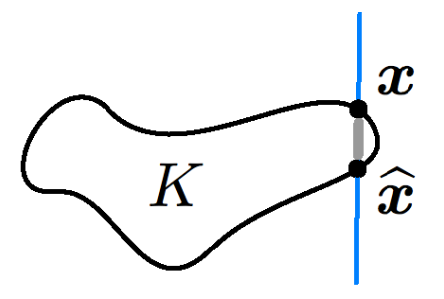
\includegraphics[scale=0.35]{Images/ch2/fig9.png}
\caption{
$\hat{\bm{x}}$
پاسخ تخمینی بردار
$\bm{x}$
از محل تقاطع 
$\mathcal{K}$
و 
زیرفضای افاین
$\bm{x}^{\prime}~:~ \bm{A}\bm{x}^{\prime}=\bm{y}$
\cite{Plan2016}}
\label{fig9}
\end{figure}


\begin{theorem}
\label{theorem:thm5}
\cite[قضیه~ ۴.۱]{vershynin2015estimation}
فرض کنید
$\mathcal{K}\subset \R^{n}$
یک مجموعه‌ی کراندار، 
$\bm{x}\in \mathcal{K}$
بردار مجهول و
$\bm{y}= \bm{A}\bm{x}$
بردار مشاهدات باشند.
با انتخاب بردار
$\hat{\bm{x}}$
با استفاده از هر تخمین‌گر که در دو رابطه‌ی
$\hat{\bm{x}}\in \mathcal{K}$
و
$\bm{y}= \bm{A}\hat{\bm{x}}$
صدق کند. رابطه‌ی زیر برقرار خواهد بود.
\begin{align}
\label{eq:eq17}
\mathbb{E}~ \sup_{\bm{x}\in \mathcal{K}} \norm{\hat{\bm{x}}-\bm{x}}_{2} \leq \dfrac{C w\left(\mathcal{K}\right)}{\sqrt{m}}
\end{align}
\end{theorem}
\begin{proof}
اثبات این قضیه در 
\cite{vershynin2015estimation}
آمده است.
\end{proof}


\subsection{تخمین با استفاده از مساله‌ی بهینه‌سازی}
در این قسمت با ساده‌تر کردن دو فرض
$\hat{\bm{x}}\in \mathcal{K}$
و
$\bm{y}= \bm{A}\hat{\bm{x}}$
، تخمین‌گر را به صورت یک مساله‌ی بهینه‌سازی در نظر می‌گیریم. علاوه بر این فرض کنید که مجموعه‌ی
$\mathcal{K}$
توپر و ستاره شکل باشد. ستاره شکل بودن به این معنا است که به ازای هر نقطه‌ی موجود در 
$\mathcal{K}$
، یک پاره خط وجود دارد که تماما در داخل مجموعه قرار دارد و از مرکز به آن نقطه متصل می‌گردد. به عبارت ریاضی:
\begin{align*}
t\mathcal{K} \subseteq \mathcal{K} \quad \text{for all} \quad t \in [0,1].
\end{align*}

برای چنین مجموعه‌ی شدنی، می‌توان با تغییر مقدار 
$t$
از صفر به سمت یک، مجموعه‌ی
$t\mathcal{K}$
را از یک نقطه تا حدی بزرگ نمود که به زیر فضای
$\bm{x}^{\prime}~:~ \bm{A}\bm{x}^{\prime}=\bm{y}$
مماس گردد. در این حالت می‌توان نقطه‌ی تماس بین مجموعه‌ی
$t\mathcal{K}$
و زیرفضا را به عنوان پاسخ تخمین‌گر در نظر گرفت. در شکل 
\ref{fig10}
این فرآیند  به صورت گرافیکی نمایش داده است.

\begin{figure}
\centering
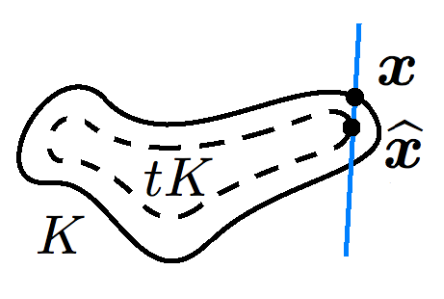
\includegraphics[scale=0.35]{Images/ch2/fig10.png}
\caption{
$\hat{\bm{x}}$
پاسخ تخمینی بردار
$\bm{x}$
از محل تقاطع 
$t\mathcal{K}$
و 
زیرفضای افاین
$\bm{x}^{\prime}~:~ \bm{A}\bm{x}^{\prime}=\bm{y}$
\cite{Plan2016}}
\label{fig10}
\end{figure}


جهت توضیح ریاضی، نیاز به تعریف تابع مینکوسکی
\LTRfootnote{Minkowski}
است. تابع مینکوسکی
به هر نقطه‌ی
$\bm{x}\in \R^{n}$
یک مقدار غیر منفی 
$\norm{\bm{x}}_{\mathcal{K}}$
اختصاص می‌دهد که به صورت زیر تعریف می‌گردد.
\begin{align}
\label{eq:eq18}
\norm{\bm{x}}_{\mathcal{K}} = \inf \lbrace \lambda >0~:~ \lambda^{-1}\bm{x}\in \mathcal{K}\rbrace
\end{align}

تابع مینکوسکی در آنالیز تابعی هندسی و آنالیز محدب پر کاربرد است. ویژگی‌های تابع مینکوسکی در مرجع 
\cite{rockafellar1970convex}
بیان شده است. در این قسمت ما تنها به صورت خلاصه به بیان خواص مورد نیاز خود می‌پردازیم. اول اینکه تابع
$\bm{x}\mapsto \norm{\bm{x}}_{\mathcal{K}}$
دارای خاصیت همگنی است (
$\norm{a\bm{x}}_{\mathcal{K}} = a \norm{\bm{x}}_{\mathcal{K}}; a>0$).
خاصیت دیگر تابع مینکوسکی
به صورت زیر بیان می‌شود.
\begin{align}
\label{eq:eq19}
\mathcal{K}= \lbrace \bm{x}~:~ \norm{\bm{x}}_{\mathcal{K}}\leq 1 \rbrace
\end{align}
در صورتی که مجموعه‌ی
$\mathcal{K}$
محدب باشد، تابع مینکوسکی
برابر با تابع نُرم خواهد بود. در قضیه‌ی
\eqref{theorem:thm6}
یک کران برای خطای حاصل از استفاده از این تخمین‌گر بیان شده است.
\begin{theorem}
\label{theorem:thm6}
\cite[قضیه~ ۴.۲]{vershynin2015estimation}
فرض کنید
$\hat{\bm{x}}$
پاسخ بهینه‌سازی زیر باشد.
\begin{align}
\label{eq:eq20}
\min \norm{\bm{x}^{\prime}}_{\mathcal{K}} \quad \text{s.t.} \quad \bm{A}\bm{x}^{\prime}= \bm{y}
\end{align}
آنگاه داریم
\begin{align}
\label{eq:eq21}
\mathbb{E}~ \sup_{\bm{x}\in \mathcal{K}} \norm{\hat{\bm{x}}-\bm{x}}_{2} \leq \dfrac{C w\left(\mathcal{K}\right)}{\sqrt{m}}
\end{align}
\end{theorem}
\begin{proof}
اثبات این قضیه در 
\cite{vershynin2015estimation}
آورده شده است.
\end{proof}

\subsection{بعد موثر}
فرض کنید در رابطه‌ی
\eqref{eq:eq21}
مقدار خطا به صورت زیر محدود گردد.
\begin{align}
\label{eq:eq22}
\mathbb{E}~ \sup_{\bm{x}\in \mathcal{K}} \norm{\hat{\bm{x}}-\bm{x}}_{2} \leq 0.01
\end{align}
در این صورت تعداد
\begin{align}
\label{eq:eq23}
m \sim O\left( w\left(\mathcal{K} \right)^{2}\right)
\end{align}
نمونه کافی خواهد بود. مقدار مربع عرض میانگین
$w\left(\mathcal{K} \right)^{2}$،
نشان دهنده‌ی عرض موثر مجموعه‌ی شدنی 
$\mathcal{K}$
است. بنابراین همانگونه که در بخش‌های مقدماتی از این فصل بیان گردید، با استفاده از ویژگی بعد موثر، می‌توان تعداد نمونه‌ی لازم جهت بازیابی صحیح را به دست آورد.

\section{نمونه‌برداری تک-بیتی از دیدگاه هندسی}
همانگونه که در فصل
\ref{ch:intro}
بیان گردید، با فرض نمونه‌برداری به صورت
\eqref{eq:eq10}،
اطلاعات دامنه از بین می‌رود. در این صورت می‌توان سیگنال مورد نظر را به صورت نرمالیزه در نظر گرفت. یعنی:
\begin{align}
\norm{\bm{x}}_{2}=1
\end{align}
در این حالت مجموعه‌ی شدنی 
$\mathcal{K}$
برابر با کره‌ی اقلیدسی واحد
$S^{n-1}$
می‌گردد. با فرض 
$\bm{a}_{i}$
به عنوان سطر 
$i$ام 
از ماتریس
$\bm{A}$
، می‌توان آن را به عنوان بردار نرمال یک ابرصفحه نیز در نظر گرفت. هر مولفه از بردار اندازه‌گیری (
$y_{i}$)
در این حالت، برابر با علامت ضرب داخلی بردار نرمال صفحه خواهد بود.
\begin{align}
y_{i} = \text{sign}(\langle\bm{a}_{i}, \bm{x}\rangle)
\end{align}
واضح است که اگر زاویه‌ی بین بردار
$\bm{x}$
و بردار نرمال صفحه از ۹۰ درجه کمتر باشد، علامت ضرب داخلی مثبت است و در غیر این صورت منفی خواهد بود. بنابراین هر نمونه، مشخص کننده‌ی یک نیم فضا خواهد بود. با اضافه شدن شرط 
$\norm{\bm{x}}_{2}=1$
فضای پاسخ به صورت بخشی از پوسته‌ی 
$S^{n-1}$
خواهد بود. در شکل
\ref{fig11}
تعبیر هندسی این مساله در فضای
$\R^{3}$
و به ازای
$m=4$
نشان داده شده است. اگر دو بردار دلخواه
$\bm{u}\in \R^{3}$
و
$\bm{v}\in \R^{3}$
بر روی 
$S^{2}$
فرض گردد، با استفاده از قضیه‌ی برش ابرصفحه‌های تصادفی می‌توان حداکثر فاصله‌ی بین دو نقطه را بر حسب تعداد نمونه‌های اخذ شده محدود نمود.

\begin{figure}
\centering
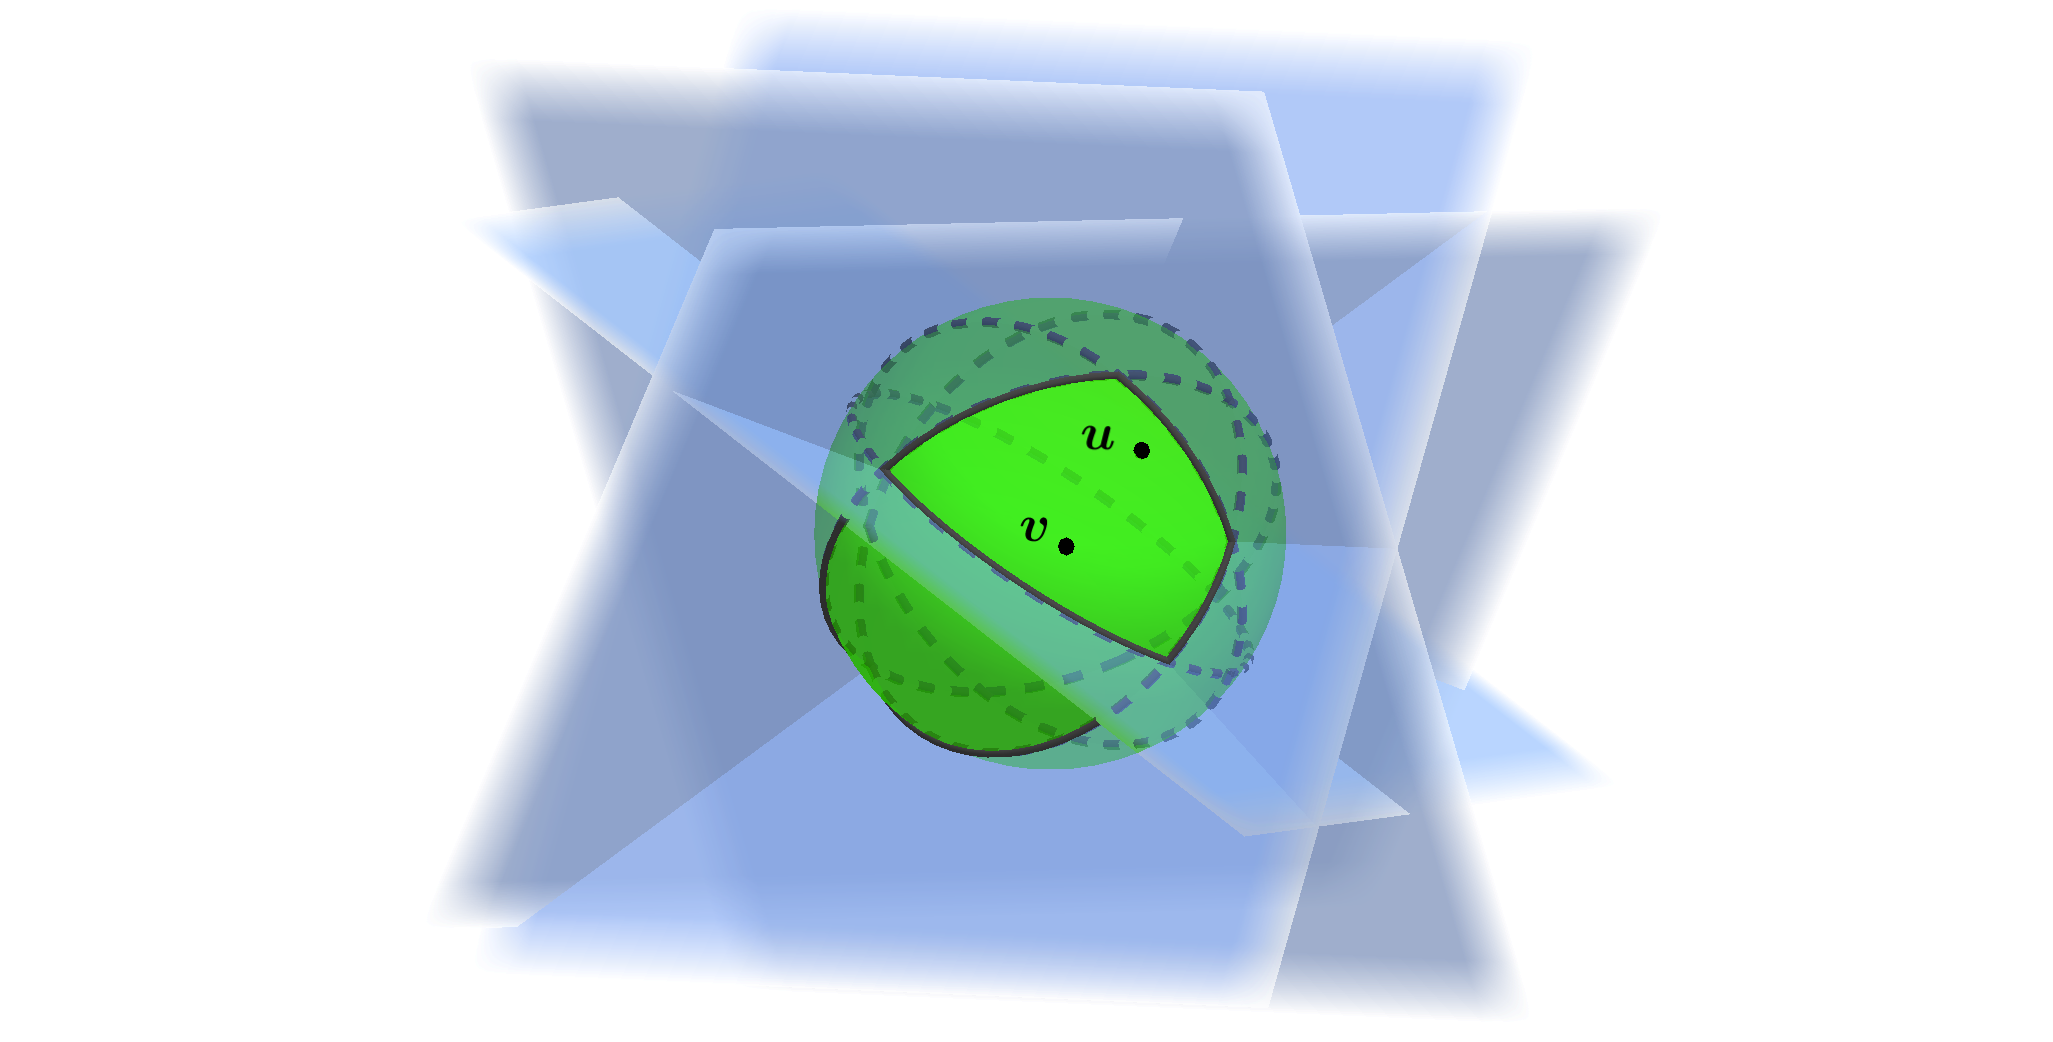
\includegraphics[scale=1.3]{Images/ch2/fig11.png}
\caption{تعبیر هندسی نمونه‌برداری تک بیتی
در 
$\R^3$
. با استفاده از قضیه‌ی برش ابرصفحه تصادفی می‌توان فاصله‌ی بین دو بردار تصادفی 
$\bm{v}$
و
$\bm{u}$
را محدود نمود.}
\label{fig11}
\end{figure}

\subsection{برش ابرصفحه تصادفی}
همانگونه که بیان گردید، هر یک از نمونه‌های باینری نشان دهنده‌ی یک نیم فضا است که با اضافه شدن شرط نرمالیزه بودن بردار، تشکیل یک مجموعه‌ی شدنی می‌دهند. سوالی که مطرح می‌گردد این است که چه تعداد نمونه‌ی جهت بازیابی سیگنال با خطای مشخص لازم است؟

در مرجع
\cite{plan2014dimension}
اندازه‌ی برش‌های تشکیل شده بر روی یک مجموعه‌ی شدنی بر حسب تعداد نمونه بررسی شده است. این مرجع، فرآیند تقسیم پوسته‌ی 
$S^{n-1}$
به برش‌های مختلف را برش ابر صفحه تصادفی
\LTRfootnote{Random Hyperplane Tessellation}
(به اختصار
\lr{RHT}
)
نامیده است.


قبل از بیان نتیجه اصلی مرجع
\cite{plan2014dimension}
، لازم است که تعریف برش 
$ \delta $-یکنواخت
را بیان نمود.

\begin{definition}
\cite[تعریف~1.1]{plan2014dimension}
\label{defn:D-UT}
فرض کنید که 
$\mathcal{K}$
یک زیر مجموعه از
$ S^{n-1} $
باشد. همچنین
$m$
ابرصفحه در
$\R^{n}$
فرض کنید. 
$ d\left(\bm{u},\bm{v}\right) $
نشان دهنده‌ی نسبت تعداد ابرصفحه‌هایی است که دو نقطه‌ی 
$ \bm{u}$
و
$\bm{y}$
در
$\mathcal{K} $
را از یکدیگر جدا می‌کند. 
مجموعه‌ی 
$\mathcal{K}$
را برش
$ \delta $-یکنواخت
می‌گوییم اگر برای یک مقدار 
$\delta >0$
رابطه‌ی زیر برقرار باشد.
\begin{align}
\label{eq:eq24}
|d\left(\bm{v},\bm{u}\right)-d_{G}\left(\bm{v},\bm{u}\right) |\leq \delta \quad \bm{u},\bm{v} \in \mathcal{K}
\end{align}
\end{definition}

با توجه به مساله‌ی مورد بررسی، با فرض سطر‌های 
$\bm{A}$
به عنوان بردار نرمال صفحات، 
$d\left(\bm{v},\bm{u}\right)$
نشان‌دهنده‌ی فاصله‌ی همینگ نرمالیزه‌ی (
$ d_{H}\left(\bm{z},\bm{t}\right)  $
)
بین
$\bm{z}:= \text{sign}\left(\bm{A}\bm{u}\right)$
و
$\bm{t}:= \text{sign}\left(\bm{A}\bm{v}\right)$
است.  در قضیه‌ی
\eqref{theorem:thm7}
تعداد نمونه‌های لازم جهت برش
$ \delta $-یکنواخت
، را بر حسب بعد موثر مجموعه‌ی
$\mathcal{K}$
محاسبه شده است.
\begin{theorem}
\label{theorem:thm7}
\cite[قضیه~1.2]{plan2014dimension}
فرض کنید
$\mathcal{K}\subset S^{n-1}$
، 
$\delta>0$
و
\begin{align*}
	m \geq C \delta^{-6} w\left(\mathcal{K}\right)^{2}
\end{align*}
باشد.
در این صورت با در نظر گرفتن یک دسته‌ی 
$m$تایی
از ابرصفحه‌های تصادفی تولید شده با توزیع یکنواخت، با احتمال 
$1-2\exp(-c\delta^{2}m)$
، این صفحات یک برش
$ \delta $-یکنواخت
از  مجموعه‌ی 
$\mathcal{K}$
ایجاد می‌کنند. 
\end{theorem}
در بخش بعدی از این پایان‌نامه با استفاده از قضیه‌ی فوق باند خطای بازیابی سیگنال‌های دیکشنری-تنک با نمونه‌های باینری، محاسبه شده است. 













\chapter{بازیابی وفقی سیگنال دیکشنری-تنک با استفاده از نمونه‌برداری تک بیتی}
\label{ch:main}
\newpage
\section{تحلیل سیگنال‌های دیکشنری-تنک}
تا این قسمت از پایان‌نامه به تحلیل و بررسی روش‌های نمونه‌برداری و بازیابی سیگنال‌های تنک پرداخته شده است. در بسیاری از کاربرد‌های عملی، سیگنال مورد بررسی مستقیما و یا در یک دسته از پایه‌های متعامد تنک نیست. در این حالت سیگنال، در یک دیکشنری غیر متعامد تنک خواهد بود.

در ادامه، سیگنال تنک را با
$ \bm{x}\in \R^N $
و دیکشنری افزونه
\LTRfootnote{Redundant}
را با 
$ \bm{D}\in \R^{n\times N} $
نشان می‌دهیم. همچنین سیگنال مورد بررسی با
$ \bm{f}\in \R^n $
 نشان داده شده که به صورت
 $ \bm{f}=\bm{D}\bm{x} $
 با پایه‌های تنک در ارتباط است. مقدار همبستگی ماتریس 
 $\bm{D}$
 به صورت زیر تعریف می‌گردد.
\begin{align}
\label{eq:eq25}
\mu := \max_{1\leq i\neq j\leq N} \dfrac{| \langle d_{i},d_{j}\rangle|}{\norm{d_{i}}_{2}\norm{d_{j}}_{2}}
\end{align}

در رابطه‌ی
\eqref{eq:eq25}
، 
$ d_{i} $
و
$ d_{j} $
نشان‌گر ستون‌های
$i$ام
و
$j$ام
از ماتریس 
$ \bm{D} $
هستند. در صورتی که مقدار
$ \mu = \mu\left(\bm{D}\right) $
کوچک باشد، دیکشنری 
$ \bm{D} $
ناهمدوس
\LTRfootnote{Incoherent}
نامیده می‌شود. با فرض
$ \bm{D} $
به صورت یک ماتریس مربعی با همبستگی پایین، حاصل‌ضرب 
$ \bm{A}\bm{D} $
گوسی است و نتایج حسگری فشرده بازیابی صحیح با استفاده از نمونه‌های
$ \bm{y}=\bm{A}\bm{f}=\bm{A}\bm{D}\bm{x} $
را تضمین می‌کند، در صورتی هدف از این گزارش سیگنال‌های تنک در دیکشنری افزونه است.

در ادامه، به صورت خلاصه دو ساختار مشابه ولی از دو کلاس متفاوت از سیگنال‌های دیکشنری تنک بررسی شده است. این دو کلاس از سیگنال‌ها، تنک-تحلیلی
\LTRfootnote{Analysis-sparse}
و تنک-ترکیبی
\LTRfootnote{Synthesis-sparse}
نامیده می‌شوند. مفاهیم اساسی سیگنال‌های تنک-تحلیلی
و  تنک-ترکیبی
در مراجع
\cite{elad2007analysis,Candes2011,nam2013cosparse}
بیان شده است. در اینجا ما تنها یک مرور خلاصه بر ایده‌ی اصلی می‌کنیم.
\begin{itemize}
\item{
سیگنال
\textbf{تنک-ترکیبی}:

برای ساخت این دسته از سیگنال‌ها، ابتدا، 
$s$
ستون (اتم) از دیکشنری 
$\bm{D}$
، به صورت تصادفی انتخاب می‌گردد (توجه داشته باشید که مجموعه‌ی اندیس‌ها با 
$ T $
نشان داده شده است.). در ادامه مقادیر دامنه‌ی 
$ s $
مولفه از بردار
$ \bm{x} $
به صورت تصادفی از یک توزیع (به عنوان مثال توزیع نرمال) انتخاب می‌گردد. سیگنال 
$ s $
-تنک ترکیبی
$ \bm{f} $
، با ضرب دیکشنری 
$\bm{D}$
در بردار 
$ \bm{x} $
به دست می‌آید.
}
\item{
سیگنال
\textbf{تنک-تحلیلی}:

جهت معرفی این دسته از سیگنال‌ها نیاز به بیان مفهوم متمم-تنکی 
\LTRfootnote{Cosparsity}
است. متمم-تنکی بردار
$ \bm{f} $
در اپراتور
$ \bm{\bm{\Omega}}\in \R^{N\times n} $
،‌ برابر با تعداد صفرهای موجود در
$ \bm{\bm{\Omega}}\bm{f} $
است. با استفاده از مفهوم متمم-تنک می‌توان سیگنال‌های تنک-تحلیلی را به عنوان دوگان تنک-ترکیبی مطرح نمود. ماتریس
$ \bm{\bm{\Omega}}\in \R^{N\times n} $
را به عنوان اپراتور تحلیلی
\LTRfootnote{Analysis operator} 
در نظر بگیرید. برای ساخت سیگنال 
$ s $
-تنک تحلیلی، ابتدا 
$l$
سطر از 
$\Omega$
را به صورت تصادفی انتخاب می‌کنیم (توجه داشته باشید که مجموعه‌ی اندیس‌ها با 
$ \Lambda $
نشان داده شده و
$\vert \Lambda \vert = l$
است). در ادامه بردار تصادفی 
$ \bm{x} $
را با درایه‌‌های
\lr{iid}
گوسی تولید می‌کنیم. سیگنال متمم-تنک با تصویر
$ \bm{x} $
بر مکمل متعامد زیرفضای تولید شده توسط 
$ \bm{\bm{\Omega}}_{\Lambda} $
به دست می‌آید. به عبارت ریاضی
\begin{align}
\label{eq:eq26}
\bm{f}= (\bm{I}-\bm{\Omega}^{\ast}_{\Lambda}(\bm{\Omega}_{\Lambda}\bm{\Omega}^{\ast}_{\Lambda})^{-1}\bm{\Omega}_{\Lambda})\bm{x}
\end{align}
در عبارت فوق، 
$ \bm{\bm{\Omega}}_{\Lambda} $
نشان‌دهنده‌ی سطرهایی از 
$ \bm{\Omega} $ 
است که در مجموعه‌ی 
$ \Lambda $
قرار دارند.
}
\end{itemize}

با دقت در تعریف سیگنال تنک-ترکیبی مشخص است که با حذف ستون‌هایی از 
$\bm{D}$
که در
$ T $
قرار دارند، زیرفضای سیگنال تغییر نمی‌کند. از طرف دیگر، در سیگنال‌های تنک-تحلیلی
مجموعه‌ی اندیس‌های متمم-تنک
($ \langle \omega_{i}, \bm{f} \rangle =0,~ i \in \Lambda $)
تعیین کننده‌ی زیرفضای سیگنال هستند.

در حالت کلی زیرفضای سیگنال‌های تنک-تحلیلی و تنک-ترکیبی با یکدیگر متفاوت هستند. با این حال، از میان تمام زیرفضا‌های مدل 
تحلیلی یکی سازنده‌ی زیرفضای  ترکیبی است. با در نظر گرفتن یکسان بودن زیرفضای سازنده‌ی سیگنال‌های
تحلیلی و
ترکیبی، شکل 
\ref{fig12}
فرآیند ساخت و نمونه‌برداری تک-بیتی از یک سیگنال دیکشنری تنک را نشان می‌دهد.

\begin{figure}
\centering
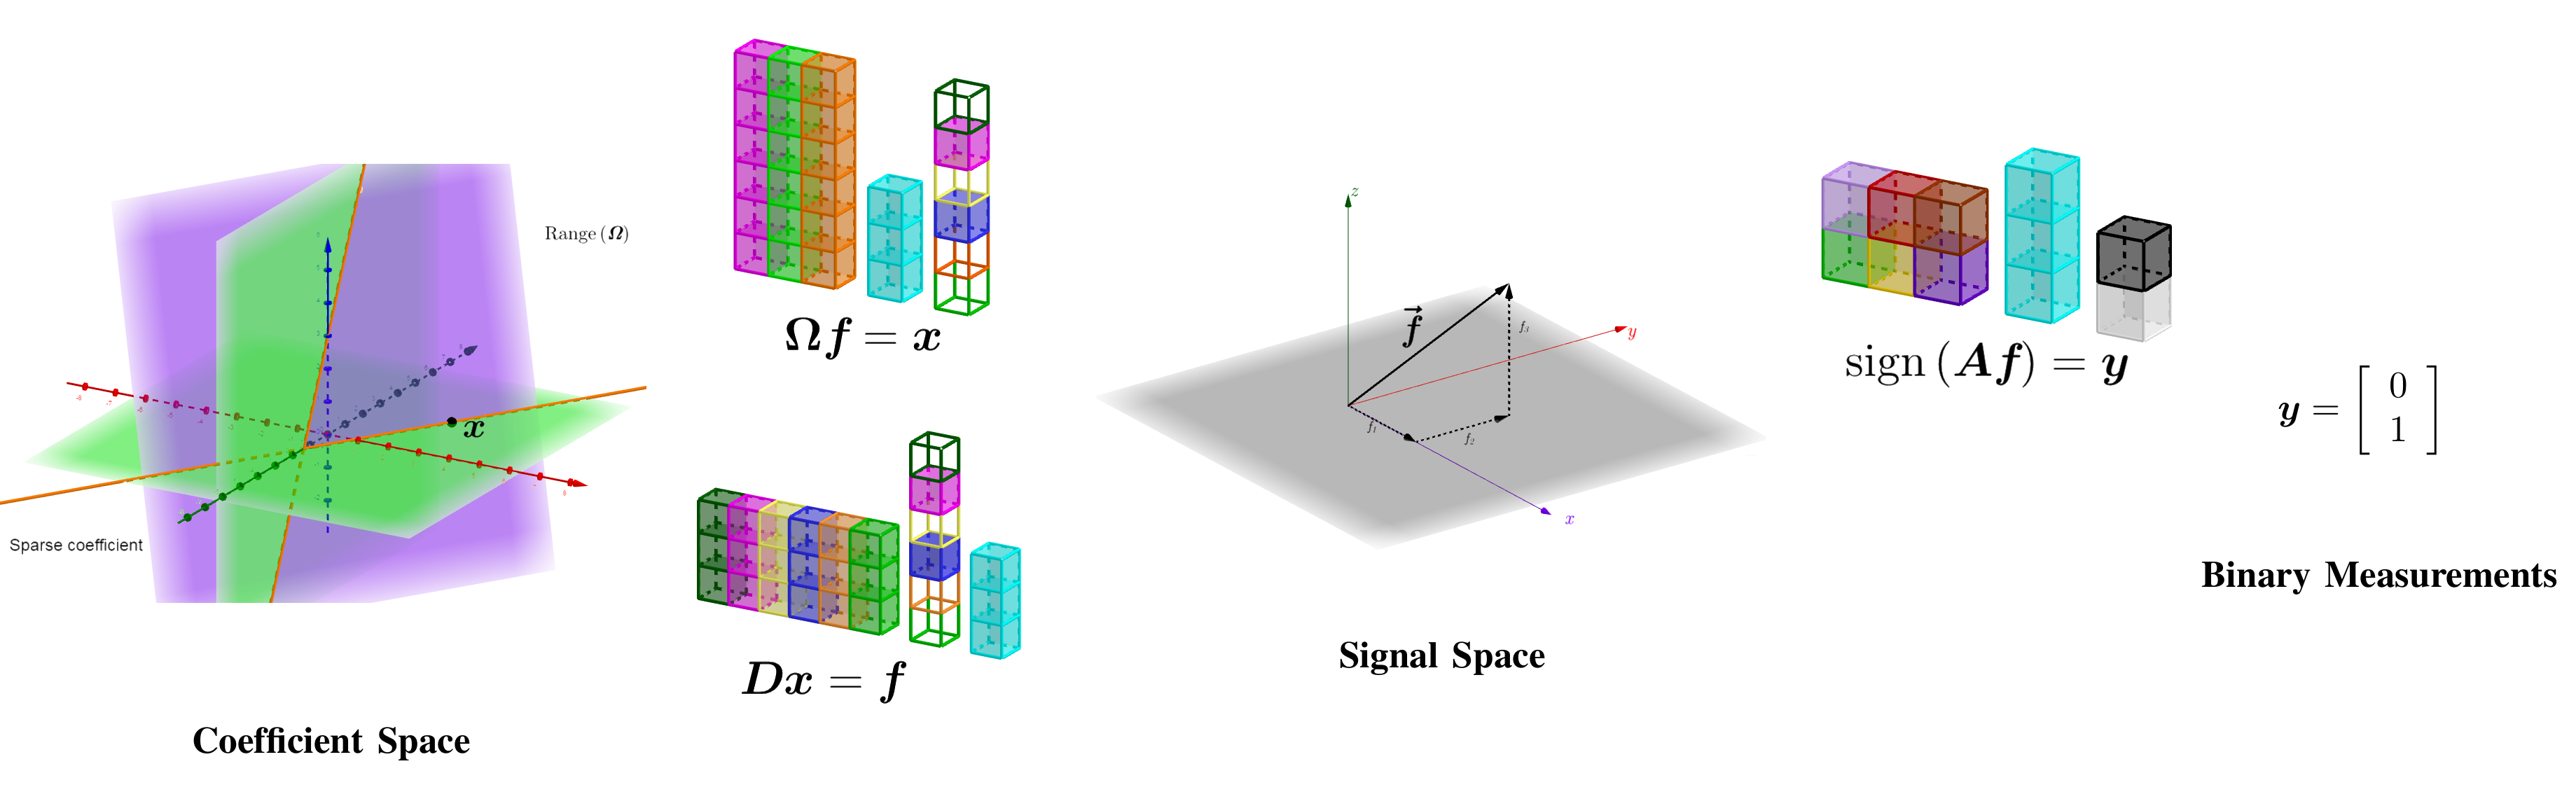
\includegraphics[scale=0.1]{Images/ch3/fig12.png}
\caption{فرآیند ساخت و نمونه‌برداری از یک سیگنال دیکشنری تنک}
\label{fig12}
\end{figure}

در این پایان‌نامه از اپراتور تحلیلی با چارچوب فشرده 
\LTRfootnote{Tight frame}
استفاده شده است. چارچوب فشرده به صورت زیر تعریف می‌گردد.
سطر‌های 
$ \bm{\Omega} $
تشکیل یک چارچوب می‌دهند اگر مقادیر
$ 0< a\leq b < \infty $
وجود داشته باشند، به گونه‌ای که 
\begin{align}
\label{eq:eq27}
a\norm{\bm{f}}^{2}_{2}\leq \norm{\bm{\Omega}\bm{f}}^{2}_{2} \leq b\norm{\bm{f}}^{2}_{2} 
\end{align}
و در صورتی که 
$ a=b $
باشد، 
$ \bm{\Omega} $ 
چارچوب فشرده نامیده می‌شود.


\section{مدل سیستم}
در این بخش مدل سیستم مورد بررسی بیان گردیده است. قبل از بیان مدل، ابتدا چند تعریف مورد استفاده در قسمت‌های بعدی بیان شده است. همچنین در این قسمت تصویر بر نیم‌کره
\LTRfootnote{Hemisphere projection}
ارائه شده است. از این تصویرسازی جهت انتقال مدل نمونه‌برداری 
\eqref{eq:eq11}
به 
\eqref{eq:eq12}
استفاده شده است. همچنین با استفاده از این تصویرسازی، یک اثبات شهودی برای قضیه‌ی اصلی این پایان‌نامه ارائه شده است.
\begin{itemize}
\item{
\textbf{تنکی موثر}\LTRfootnote{Effective sparsity}


نامساوی کوشی-شوارتز مقدار نُرم
$ l_1 $
و 
$ l_2 $
سیگنال 
$ \bm{x}\in \R^{N} $
را به صورت 
$ \norm{\bm{x}}_{1}\leq \sqrt{N}\norm{\bm{x}}_{2} $
با یکدیگر مرتبط می‌کند.
بردار 
$ \bm{x}\in \R^{N} $
$s$-تنک موثر
نامیده می‌شود اگر در شرط زیر صدق کند.
\begin{align}
\label{eq:eq28}
\norm{\bm{x}}_{1}\leq \sqrt{s}\norm{\bm{x}}_{2}
\end{align}
جهت روشن شدن موضوع، مجموعه‌ی تنک موثر
$ \mathcal{K} \in S^{n-1}\cap \sqrt{s}B^{n}_{1} $
را فرض کنید. اگر درجه‌ی تنکی از
$1$
به 
$N$
افزایش یابد، توپ 
$l_1$
از یک چند وجهی محیطی که در ابتدا تنها شامل محورها است، به یک چند وجهی محاطی که شامل 
$ S^{n-1} $
است تبدیل می‌شود. طی این فرآیند با افزایش مقدار
$s$
نقاط اطراف محور‌ها به مجموعه اضافه می‌گردند. جهت نمایش سیگنال‌های 
$s$-تنک
از نماد
$ \Sigma^{N}_{s} $
و برای نمایش سیگنال‌های 
$s$-تنک موثر
از نماد 
$ \Sigma^{N,\text{eff}}_{s} $
استفاده شده است.

اگر سیگنال مورد بررسی از یک دیکشنری تنک انتخاب شده باشد، می‌گوییم که سیگنال
$ \bm{f} $
، 
$ s $
تنک ترکیبی موثر است اگر
$ \bm{f}=\bm{D}\bm{x} $
و برای یک 
$ \bm{x}\in \Sigma^{N,\text{eff}}_{s} $،
$ s $
تنک تحلیلی موثر است اگر
$ \bm{D}^{\ast}\bm{f}\in \Sigma^{N,\text{eff}}_{s} $
باشد.
}
\item{\textbf{مجموعه‌ی پیش-تصویر}
\LTRfootnote{Pre-image set}

برای یک ماتریس (معکوس‌ناپذیر)
$ \bm{D} $
، نماد
$ \bm{D}^{-1}(\mathcal{K}) $
نشان دهنده‌ی مجموعه‌ی پیش-تصویر 
$ \mathcal{K} $
است. به عنوان مثال اگر به ازای
$\bm{f}\in \mathcal{K} $
،
$\bm{f}= \bm{D}\bm{x}$
باشد، آنگاه 
$\bm{x}$
عضو مجموعه‌ی پیش-تصویر 
$\mathcal{K}$
یا
$ (\bm{D}^{\ast})^{-1}(\mathcal{K})$
است.  در موضوع مورد بحث، مجموعه‌ی پیش تصویر
$ \bm{D}^{\ast} $
برای حالت تحلیلی
برابر با
$ \text{Range}(\bm{\Omega}) $
و برای حالت ترکیبی برابر با
$ \text{Span}(\bm{x}) $
است.
}
\end{itemize}

\begin{definition}[تصویر بر نیم‌کره]
\label{defn:HP}
فرض کنید
$ \bm{f}\in \R^{N} $
یک سیگنال اختیاری و
 $ \sigma >0 $
برابر با شعاع نیم‌کره باشد.
سیگنال منتقل شده‌ی
\LTRfootnote{lifted}
$ \bm{f} $
را به صورت
$ \tilde{\bm{f}}:= [\bm{f}^{T}~|~\sigma]^{T}\in \R^{N+1} $ 
تعریف می‌کنیم. تصویر سیگنال انتقال یافته بر نیم‌کره به شعاع
$\sigma$
 به صورت زیر محاسبه می‌گردد.

\begin{align}
\label{eq:eq29}
P_{\sigma}(\tilde{\bm{f}}) =\sigma \dfrac{\tilde{\bm{f}}}{\|\tilde{\bm{f}}\|_{2}}
\end{align}
\end{definition}

\begin{figure}[t]
	\centering
	\begin{subfigure}{0.4\textwidth} % width of left subfigure
		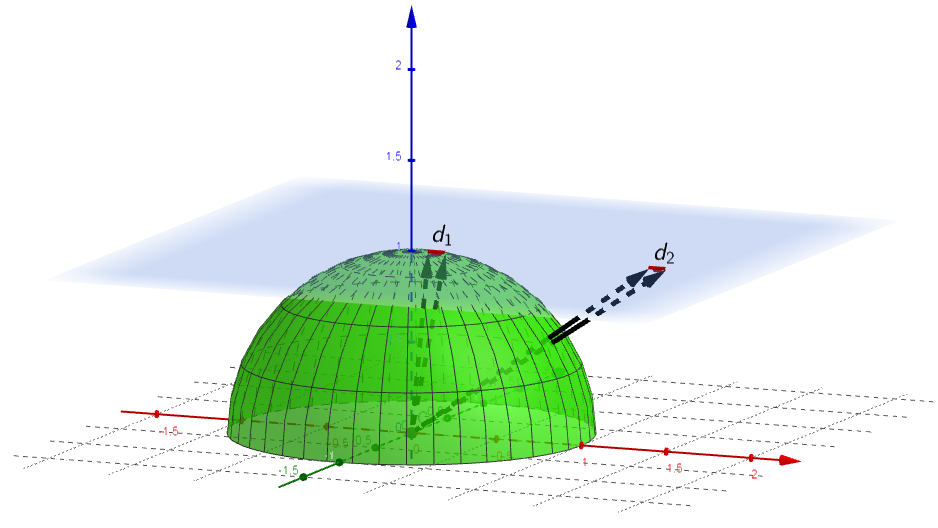
\includegraphics[scale=0.2]{Images/ch3/fig13.png}
		\caption{} % subcaption
		\label{fig13}
	\end{subfigure}
	\vspace{1em} % here you can insert horizontal or vertical space
	\begin{subfigure}{0.4\textwidth} % width of right subfigure
		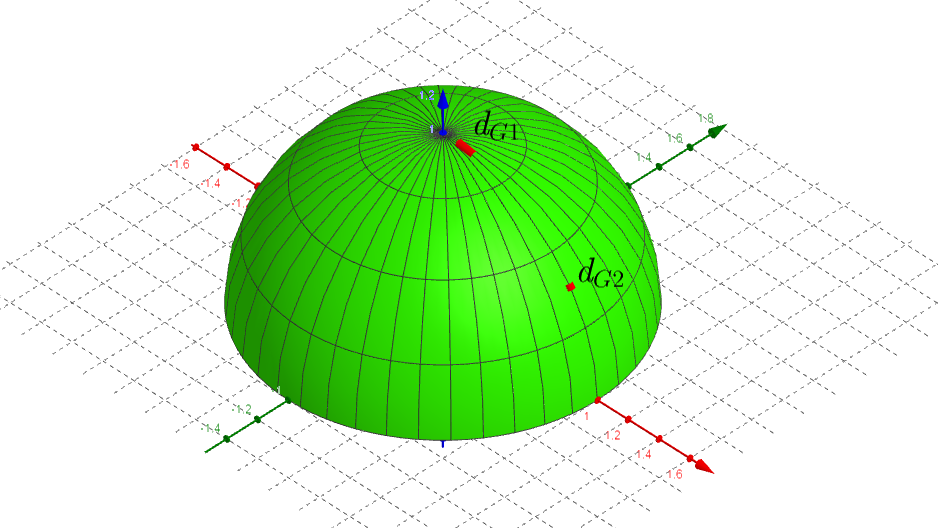
\includegraphics[scale=0.2]{Images/ch3/fig14.png}
		\caption{} % subcaption
		\label{fig14}
	\end{subfigure}
	\caption{تعبیر هندسی تصویر بر نیم‌کره}
\end{figure}

اگرچه تعریف 
\eqref{defn:HP}
بسیار ساده است ولی تعبیر هندسی آن در فهم مساله‌ی ما بسیار موثر است. نکته‌ی بسیار مهم در تعریف
\eqref{defn:HP}
این است که این نگاشت فاصله‌ی بین نقاط را حفظ نمی‌کند. جهت روشن شدن این موضوع به مثال زیر توجه کنید.

فرض کنید 
$ \bm{f}_{1}=[0.1,0,0]^{T} $
،
$ \bm{f}_{2}=[0.2,0,0]^{T} $
،
$ \bm{f}_{3}=[1,0,0]^{T} $
و 
$ \bm{f}_{4}=[1.1,0,0]^{T} $
چهار نقطه از فضای سه بعدی بر روی صفحه‌ی
$ z=1 $
باشند. کاملا واضح است که فاصله‌ی بین 
 $ \bm{f}_{1} $
و
 $ \bm{f}_{2} $
برابر با فاصله‌ی بین
 $ \bm{f}_{3} $
و 
 $ \bm{f}_{4} $
و مساوی با
$ d_{1}=\norm{\bm{f}_{1}-\bm{f}_{2}}_{2}=d_{2}=\norm{\bm{f}_{3}-\bm{f}_{4}}_{2}= 0.1 $
است. در این مثال شعاع نیم‌کره را
$ \sigma =1  $
و مرکز آن را
$ [0,0,0]^{T} $ 
در نظر می‌گیریم (شکل
\ref{fig13}
).
در ادامه نقاط را بر روی نیم‌کره تصویر می‌کنیم (شکل
\ref{fig14}
). فاصله‌ی ژئودزیک بین نقاط تصویر شده به صورت زیر محاسبه می‌گردند.
\begin{align*}
	 d_{G1}&=d_{G}(P_{\sigma}(\tilde{\bm{f}}_{1}),P_{\sigma}(\tilde{\bm{f}}_{2}))= 0.0311\\
	 d_{G2}&=d_{G}(P_{\sigma}(\tilde{\bm{f}}_{3}),P_{\sigma}(\tilde{\bm{f}}_{4}))= 0.0103.
\end{align*}

تفاوت در اندازه‌های تصویر شده با افزایش مقدار نُرم 
$l_2$
افزایش می‌یابد. در کاربرد مورد استفاده‌ی ما با تغییر شعاع نیم‌کره به اندازه‌ی مناسب این تفاوت کنترل شده است.

پس از بیان تعاریف مورد نیاز در قسمت‌های بعدی در این قسمت مدل سیستم بررسی شده است.
فرض کنید، 
$ \bm{f}\in \R^{n} $
یک سیگنال
$s$-تنک ترکیبی
 یا
$s$-تنک تحلیلی
و 
$ \bm{A} $
ماتریس اندازه‌گیری باشد.
بر خلاف روش‌های موجود جهت بازیابی سیگنال‌های دیکشنری-تنک با استفاده از نمونه‌های تک-بیتی که در یک مرحله و با یک تنظیمات تمامی نمونه‌ها را اخذ می‌کند، ما این فرآیند را در چند مرحله انجام می‌دهیم. در این کار آستانه‌ها در طی روند نمونه‌برداری و با استفاده از اطلاعات نمونه‌های قبلی، به صورت وفقی تغییر می‌کند. توجه داشته باشید که ماتریس
$ \bm{A} $
به صورت تصادفی ایجاد شده است ولی در طی روند نمونه‌برداری ثابت فرض می‌شود. همچنین جهت تعریف آستانه‌ها از آستانه‌های ابعاد بالا 
$ \bm{\varphi}^{(i)}\in \R^{n} $
استفاده شده است.
 شکل 
\ref{fig15}
بلوک دیاگرام سیستم مورد بررسی را نشان می‌دهد.
\begin{figure}
	\centering
	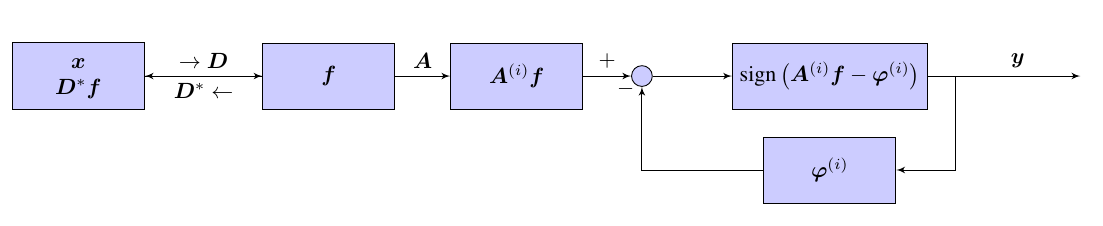
\includegraphics[scale=0.4]{Images/ch3/fig15}
	\caption{بلوک دیاگرام مدل نمونه‌برداری وفقی سیگنال‌های دیکشنری تنک}
	\label{fig15}
\end{figure}

\subsection{بازیابی تک مرحله‌ای}
در روش پیشنهادی، از نتایج به دست آمده در مراحل میانی، جهت بهبود فرآیند وفقی استفاده شده است. در این بخش، هر مرحله از الگوریتم به صورت جداگانه بررسی شده است. هر مرحله از الگوریتم را بازیابی تک مرحله‌ای
\LTRfootnote{Single step recovery}
می‌نامیم. در بازیابی تک مرحله‌ای، در مرحله‌ی 
$i$ام
 ، ماتریس اندازه‌گیری
 $ \bm{A} $
 و آستانه برابر با
 $ \bm{\tau} $
 است.
 قضیه‌ی 
 \ref{theorem:thm8}
 رابطه‌ی بین خطای بازیابی و تعداد نمونه‌ها در بازیابی تک مرحله‌ای را نشان می‌دهد.
 
\begin{theorem}
\label{theorem:thm8}
فرض کنید
$ \epsilon,r,\sigma,C,c^{\prime},\gamma >0 $
و درایه‌های
$ \bm{A}\in \R^{m\times n} $
 از توزیع استاندارد نرمال انتخاب شده باشند. همچنین فرض کنید
 $ \tau_{i}~ i=1,\cdots,m $
 از توزیع گوسی با میانگین صفر و واریانس 
$ \sigma^{2} $
و به صورت مستقل از
$ \bm{A} $
انتخاب شده باشند. با فرض سیگنال
$ \bm{f}\in \R^{n} $
به عنوان یک سیگنال 
$ s $-تنک
تحلیلی(ترکیبی)
در دیکشنری
$\bm{D}\in \R^{n\times N}$
با 
$ \|\bm{f}\|_{2}\leq r $
و
$ \|\bm{D}^{\ast}\bm{f}\|_{1}\leq \sqrt{s} r $
، اگر ما تعداد
$ m \geq C(r/\sigma+\sigma / r)^{6}(r^{2}/\sigma^2+1)\epsilon^{-6}s \log (N/s) $ 
نمونه با استفاده از مدل نمونه‌برداری
\eqref{eq:eq12}
دریافت کنیم، با احتمال حداقل
$ 1-\gamma \exp{(-c^{\prime}m \epsilon^{2} r^2\sigma^2/ (r^2+\sigma^2)^2)} $
پاسخ
\begin{align}
\label{eq:SSR}
 \bm{f}_{\varDelta}~=~\mathop{\arg\min}_{\bm{h}\in \R^{n} } \norm{\bm{D}^{*}\bm{h}}_{1}\quad \text{s.t.} \quad   \bm{y} = \text{sign}\left(\bm{A}\bm{h}-\bm{\tau}\right), \: \norm{\bm{h}}_{2}\leq r,
\end{align}
 در شرط زیر صدق خواهد نمود:
\begin{align}
\|\bm{f}-\bm{f}_{\varDelta}\|_{2}\leq \epsilon r
\end{align}
\end{theorem}
\begin{proof}
اثبات این قضیه در 
\ref{Appndx1}
آورده شده است.
\end{proof}

\section{نتایج اصلی}

\subsection{آستانه‌ی ابعاد بالا}
الگوریتم پیشنهادی جهت تولید آستانه‌های ابعاد بالا در الگوریتم
\ref{alg:HDTG}
آورده شده است. خروجی الگوریتم شامل دو بخش است. بخش اول، یک نقطه‌ی مشخص در فضای سیگنال است که با استفاده از پاسخ تقریبی مرحله‌ی قبل از نمونه‌برداری محاسبه می‌گردد. این نقطه مرکز مجموعه‌ای است که قصد داریم با نمونه‌برداری آن را برش دهیم (در مرحله‌ی اول از الگوریتم این نقطه برابر با مبدا است.). 


\begin{algorithm}
	\caption{$ \Phi $: مولد آستانه در ابعاد بالا}
	\label{alg:HDTG}
	\begin{algorithmic}[1]
		\renewcommand{\algorithmicrequire}{\textbf{ورودی:}}
		\renewcommand{\algorithmicensure}{\textbf{خروجی:}}
		\REQUIRE ماتریس اندازه‌گیری $ \bm{A} $, تعداد نمونه‌ها $ b $, واریانس لغزش‌ها $ \sigma^{2} $, سیگنال تخمینی $ \hat{\bm{f}} $.
		\ENSURE بردار آستانه در ابعاد بالا $\bm{\varphi}\in \R^{b}$.
		\STATE $ \bm{\tau}\sim N(0,\sigma^{2}\bm{I}_{b} ) $
		\STATE  $ \bm{\varphi}=\bm{A}\hat{\bm{f}}+\bm{\tau} $
	\end{algorithmic} 
\end{algorithm}


در روش‌های سنتی آستانه‌گذاری، تنها پارامتر قابل کنترل، واریانس توزیع تصادفی جهت تولید آستانه‌ها است. با تغییر مقدار واریانس تنها فاصله‌ی میانگین از مبدا افزایش می‌یابد. جهت مشخص شدن تفاوت روش پیشنهادی با روش‌های موجود، یک مثال در فضای
$\R^{2}$
آورده شده است.

فرض کنید
$ \bm{A}\in \R^{4\times 2} $
ماتریس نمونه‌برداری و
$ \bm{\bm{\tau}_{1}} \sim N(0,\sigma_{1}^{2}\bm{I}_{4})$
و
$ \bm{\bm{\tau}_{2}}\sim N(0,\sigma_{2}^{2}\bm{I}_{4}) $
دو بردار لغزش
\LTRfootnote{Dither}
با
$ \sigma_{2}< \sigma_{1} $
باشد.
همچنین فرض کنید
$ \bm{f} $
سیگنال مجهول باشد. نتیجه‌ی استفاده از مدل نمونه‌برداری سنتی در شکل 
\ref{fig16}
نشان داده شده است. در صورتی که با استفاده از آستانه‌ی ابعاد بالا و تخمین اولیه‌ی 
$\hat{\bm{f}}$
می‌توان با تعداد نمونه‌ی برابر به خطای بازیابی کمتری دست یافت (شکل
\ref{fig17}
)

\begin{figure}
	\centering
	\begin{subfigure}{0.4\textwidth} % width of left subfigure
		\centering
		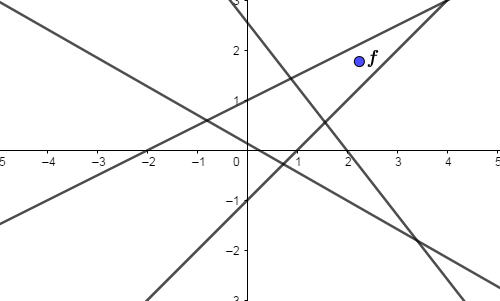
\includegraphics[scale=0.3]{Images/ch3/fig16}
		\caption{} % subcaption
		\label{fig16}
	\end{subfigure}
	\vspace{1em} % here you can insert horizontal or vertical space
	\begin{subfigure}{0.4\textwidth} % width of right subfigure
		\centering
		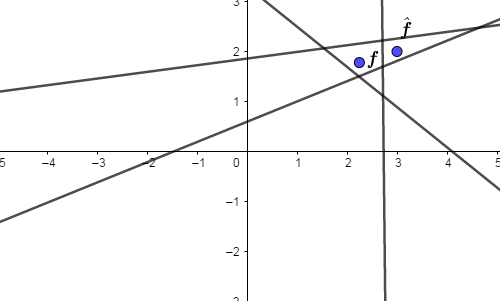
\includegraphics[scale=0.3]{Images/ch3/fig17}
		\caption{} % subcaption
		\label{fig17}
	\end{subfigure}
	\caption{نمایش هندسی تفاوت آستانه‌ی معمولی با آستانه‌ی ابعاد بالا در فضای دو بعدی}
\end{figure}


\subsection{کران خطا}
هدف اصلی از این پایان‌نامه ارائه‌ی یک الگوریتم با آستانه‌گذاری وفقی و مبتنی بر برنامه‌ریزی محدب جهت دست‌یابی به نرخ کاهش نمایی در خطای بازیابی بر حسب تعداد نمونه است. ثابت خواهیم کرد که با استفاده از آستانه‌گذاری ابعاد بالا و الگوریتم‌های نمونه‌برداری و بازیابی مناسب (الگوریتم
\ref{alg:AQ}
و
\ref{alg:AR}
)
قضیه‌ی زیر برقرار است.
\begin{theorem}
\label{thm.main}

الگوریتم‌های نمونه‌برداری و بازیابی وفقی
$ \mathcal{Q} $
و
$ \mathcal{R} $
 ( الگوریتم
\ref{alg:AQ}
و
\ref{alg:AR})
با پارامترهای
$\bm{A}\in \R^{m\times n}$،
$\bm{D}\in \R^{n\times N}$،
$\sigma$،
$r$
و
$L$
 را در نظر بگیرید. همچنین فرض کنید که آستانه‌های مورد نیاز الگوریتم‌ها با استفاده از الگوریتم
$ \Phi $
(الگوریتم
\ref{alg:HDTG})
به  دست آمده باشند. 
فرض کنید
\begin{align}
 m \geq C(r/\sigma+\sigma / r)^{6}(r^{2}/\sigma^2+1)(1/2)^{-6}s \log (N/s) 
\end{align} 
 نمونه از سیگنال
$ \bm{f}\in (\bm{D}^{\ast})^{-1} \Sigma_{s}^{N,\text{eff}} $ 
به صورت
\begin{align}
\label{eq:SignAT}
y_{i}= \text{sign}\left(\langle \bm{a}_{i},\bm{x}\rangle-\bm{\varphi}^{\left(i\right)}\right),
\end{align}

دریافت شده باشد. آنگاه خروجی الگوریتم بازیابی وفقی
$ \mathcal{R} $ 
با احتمال حداقل
\begin{align}
 1-\gamma \exp{(-c^{\prime}m (1/2)^{2} r^2\sigma^2/ (r^2+\sigma^2)^2)} 
\end{align}

در شرط 
\begin{align}
\|\bm{f}-\hat{\bm{f}}\|_{2}\leq r2^{1-L},
\end{align}
 صدق می‌کند.
\end{theorem}
\begin{proof}
یک تعبیر شهودی در 
\ref{proof:IntuitiveMain}
آورده شده است. اثبات ریاضی در پیوست
\ref{Appndx2}
موجود است.
\end{proof}



\subsection{الگوریتم نمونه‌برداری وفقی}
الگوریتم نمونه‌برداری وفقی پیشنهادی به صورت الگوریتم
\ref{alg:AQ}
نشان داده شده است. جهت اجرای این الگوریتم، نیازمند دیکشنری
$ \bm{D} $ 
(دیکشنری که سیگنال
$ \bm{f} $
در آن تنک است.)، ماتریس نمونه‌برداری
$ \bm{A} $
، نمونه‌های خطی
$ \bm{A}\bm{f} $
و یک باند بالای تخمینی از نُرم سیگنال 
$ r $
(
$ \norm{\bm{f}}_{2}\leq r $
) هستیم.
در اولین مرحله از اجرای الگوریتم، مقدار سیگنال تخمینی را صفر در نظر می‌گیریم
($ \hat{\bm{f}}=0 $).
با انتخاب تعداد مراحل تکرار الگوریتم
$ L $
، ماتریس نمونه‌برداری و بردار نمونه‌ها را به 
$ L $
بلوک تقسیم می‌کنیم. در این صورت می‌توانیم فرآیند نمونه‌برداری را آغاز کنیم.


نمونه‌برداری وفقی شامل ۳ مرحله‌ی اصلی است. ابتدا در مرحله‌ی اول،
آستانه‌های ابعاد بالا با استفاده از الگوریتم
\ref{alg:HDTG}
تولید می‌شوند. سپس در مرحله‌ی دوم، بلوک 
$i$ام
از نمونه‌های خطی با آستانه‌ی تولید شده مقایسه می‌گردد و بلوک 
$i$ام
از نمونه‌های تک بیتی تولید می‌شود. در مرحله‌ی بعدی مقدار تخمینی از سیگنال
($\hat{\bm{f}}$)،
با اجرای الگوریتم بازیابی تک-مرحله‌ای بر روی داده‌های بلوک محاسبه می‌گردد. این فرآیند تا مرحله‌ی 
$L$ام
تکرار می‌گردد. جهت افزایش سرعت همگرایی مقدار تخمین زده شده به مقدار اصلی سیگنال، در هر مرحله واریانس بخش تصادفی از آستانه‌های ابعاد بالا، نصف می‌گردد.
در نهایت الگوریتم
\ref{alg:AQ}
مقادیر نمونه‌های تک-بیتی و آستانه را به خروجی می‌فرستد.

\begin{algorithm}
	\caption{$ \mathcal{Q} $: نمونه‌برداری وفقی}
	\label{alg:AQ}
	\begin{algorithmic}[1]
		\renewcommand{\algorithmicrequire}{\textbf{ورودی:}}
		\renewcommand{\algorithmicensure}{\textbf{خروجی:}}
		\REQUIRE دیکشنری $ \bm{D}\in\R^{n\times N} $, ماتریس نمونه‌برداری $ \bm{A}\in\R^{m\times n} $, مشاهدات خطی $ \bm{Af}\in \R^{m} $, تخمین نُرم $ \norm{\bm{f}}_{2}\leq r $, تعداد بلوک‌ها $ L $, $\varDelta$: بازیابی تک مرحله‌ای \eqref{eq:SSR}.
		\ENSURE  نمونه‌های کوانتیزه $ \bm{y} \in \lbrace\pm 1\rbrace^{m} $, آستانه‌ها در ابعاد بالا $ \bm{\varphi} \in \R^{m} $
		\\ \textit{مقدار‌دهی اولیه} : $ \bm{f}_{0}\leftarrow \bm{0} $, $ b = \lfloor\frac{m}{L}\rfloor $, $ \bm{A}^{(i)}\in \R^{b\times m}  $
		\begin{latin}
		\FOR {$i = 1,\cdots,L$}
		\STATE $r_{t}=2^{1-t}r$
		\STATE $\bm{\varphi}^{\left(i\right)}\leftarrow \Phi(\bm{A}^{(i)},b,2^{1-t}r,\bm{f}_{i-1}) $
		\STATE $ \bm{y}^{\left(i\right)} = \text{sign}\left(\bm{A}^{(i)}\bm{f}-\bm{\varphi}^{\left(i\right)}\right)$
		\STATE $ \bm{f}_{i} = \bm{f}_{i-1} + \varDelta\left(\bm{D},\bm{A}^{(i)},\bm{y}^{\left(i\right)},\bm{\varphi}^{\left(i\right)},\bm{r}_{t}\right) $
		\ENDFOR
		\end{latin}
	\end{algorithmic} 
\end{algorithm}




\subsection{الگوریتم بازیابی وفقی}
در فرآیند بازیابی (الگوریتم
\ref{alg:AR})
نیازمند دیکشنری
$ \bm{D} $
ماتریس نمونه‌برداری
$ \bm{A} $
بردار نمونه‌های تک بیتی
$ \bm{y} $
بردار آستانه‌های ابعاد بالا
$ \bm{\varphi} $
و یک باند بالای تخمینی از نُرم سیگنال
$ r $
، هستیم. پس از اعمال مقادیر فوق به عنوان ورودی الگوریتم
\ref{alg:AR}
،‌ می‌توان الگوریتم را اجرا نمود. در روند اجرای بازیابی وفقی، با تقسیم بردار اندازه‌گیری،‌ نمونه‌ها و آستانه‌ها به 
$ L $
بلوک آغاز می‌گردد. در هر مرحله از اجرای الگوریتم، تنها الگوریتم بازیابی تک مرحله‌ای به ازای ورودی‌های مختلف اجرا می‌گردد.



\begin{algorithm}
	\caption{$ \mathcal{R} $: بازیابی وفقی}
	\label{alg:AR}
	\begin{algorithmic}[1]
		\renewcommand{\algorithmicrequire}{\textbf{ورودی:}}
		\renewcommand{\algorithmicensure}{\textbf{خروجی:}}
		\REQUIRE دیکشنری $ \bm{D}\in\R^{n\times N} $, ماتریس نمونه‌برداری $ \bm{A}\in\R^{m\times n} $, نمونه‌های کوانتیزه $ \bm{y} \in \lbrace\pm 1\rbrace^{m} $, آستانه‌ها در ابعاد بالا $ \bm{\varphi}\in\R^{m} $, تخمین نُرم $ \norm{\bm{f}}_{2}\leq r $, تعداد بلوک‌ها $ L $، $\varDelta$: بازیابی تک مرحله‌ای \eqref{eq:SSR}.
		\ENSURE  تخمین سیگنال $ \hat{\bm{f}}\in \R^{n} $.
		\\ \textit{مقداردهی اولیه} :  $ b = \lfloor\frac{m}{L}\rfloor $, $ \bm{A}^{(i)}\in \R^{b\times m}$, $ \bm{y}^{\left(i\right)} \lbrace\pm 1\rbrace^{b}$, $\bm{\varphi}^{\left(i\right)}\in \R^{b} $
		\begin{latin}
		\FOR {$i = 1,\cdots,L$}
		\STATE $ \bm{f}_{i} =\bm{f}_{i-1}+ \varDelta\left(\bm{D},\bm{A}^{(i)},\bm{y}^{\left(i\right)},\bm{\varphi}^{\left(i\right)},\bm{r}_{t}\right) $ 
		\ENDFOR
		\end{latin}
	\end{algorithmic} 
\end{algorithm}


نکته‌ی قابل توجه در الگوریتم بازیابی وفقی تکرار عملیات‌ها است. اگر دوباره به الگوریتم نمونه‌برداری وفقی نگاه کنیم، متوجه می‌شویم که الگوریتم 
\ref{alg:AR}
یک بخش از الگوریتم 
\ref{alg:AQ}
است. برتری الگوریتم بازیابی وفقی این است که نیاز به بردار نمونه‌های خطی
($\bm{A}\bm{f}$)
 ندارد و تنها با استفاده از نمونه‌های تک بیتی می‌تواند بازیابی سیگنال را انجام دهد. این موضوع، در صورتی که بین محل نمونه‌برداری و بازیابی فاصله باشد کاربرد خواهد داشت. به عبارت دیگر از الگوریتم نمونه‌برداری وفقی می‌توان به عنوان یک کدگذار
 \LTRfootnote{Encoder}
  و از الگوریتم بازیابی وفقی به عنوان کدگشا
 \LTRfootnote{Decoder}
 استفاده نمود. در این حالت با توجه به اینکه نمونه‌ها تک بیتی هستند حجم داده‌ی مورد نیاز جهت انتقال به شدت کاهش خواهد یافت.

\subsection{تعبیر شهودی قضیه‌ی ۹}
\label{proof:IntuitiveMain}
در این بخش، اثبات شهودی برای قضیه‌ی
\ref{thm.main}
آورده شده است. قبل از شروع اثبات، بهتر است که یک مرور سریع بر صورت قضیه داشته باشیم.

به صورت خلاصه در این قضیه، ما الگوریتم بازیابی تک مرحله‌ای را برای مقدار لغزش و مرکز مختلف، طی 
$L$
مرحله اجرا می‌کنیم. جهت اثبات این قضیه از نتایج حسگری فشرده‌ی تک بیتی سنتی استفاده شده است. تصویر بر نیم‌کره (تعریف
\ref{defn:HP}
)
در اینجا نقش پل بین حسگری فشرده تک بیتی سنتی و نتایج ارائه شده در این پایان‌نامه را بازی می‌کند.

یک نیم کره با شعاع 
$\sigma$
و مرکز مبدا مختصات در نظر بگیرید. این نیم کره در نقطه‌ی 
$ [\bm{0}^{T}~|~\sigma]^{T}\in \R^{n+1} $
به فضای سیگنال
$ \bm{f} $ 
مماس است. به خاطر آورید که هر سطر از ماتریس 
$\bm{A}$
مشخص کننده‌ی بردار نرمال یک ابرصفحه در فضای
$ \R^{n} $
است. هر کدام از این ابرصفحه‌ها را می‌توان به صورت یک ابرصفحه‌ی دیگر که از مبدا مختصات در فضای 
$ \R^{n+1} $
عبور می‌کند در نظر گرفت. در چنین شرایطی، پس از تصویر نمودن فضای سیگنال بر نیم‌کره، فضای جدید برابر با نیمه‌ی بالایی 
 $ \sigma S^{n} $
است که توسط تعداد مشخصی از ابرصفحه‌ها برش داده شده است.

همان‌گونه که در قسمت‌های قبلی بیان گردید،  الگوریتم با یک مقدار تخمین از نُرم سیگنال
$ \norm{\bm{f}}_{2} $
آغاز می‌گردد. تعبیر هندسی این انتخاب این است که در ابتدای کار، نقاطی که در فاصله‌ی دورتر نسبت به نقطه‌ی تماس قرار دارند، به نقاط مناسب از نیم‌کره تصویر می‌گردند. این موضوع باعث می‌شود که پاسخ تقریبی به دست آمده در مراحل اولیه از دقت مناسب برخوردار باشد. در هر مرحله از الگوریتم نمونه‌برداری، با استفاده از الگوریتم آستانه‌گذاری ابعاد بالا،(الگوریتم
\ref{alg:HDTG})
نقطه‌ی تماس نیم‌کره با فضای سیگنال
$ \bm{f} $ 
به محل سیگنال تخمین زده شده جابجا می‌شود و با کاهش شعاع نیم‌کره که معادل با کاهش واریانس مقادیر لغزش است، با دقت بیشتری نمونه‌های جدید را اخذ می‌کند. این فرآیند منجر به نمونه‌برداری با کیفیت بهتر می‌شود و به همین دلیل خطای بازیابی کاهش می‌یابد.















\chapter{نتایج شبیه‌سازی و پیشنهادات}
\label{simulation}
\newpage

\section{شبیه‌سازی}
در این قسمت کارایی الگوریتم پیشنهادی در این پایان‌نامه با الگوریتم‌های موجود جهت بازیابی سیگنال‌های دیکشنری تنک  
(الگوریتم‌های موجود در 
\cite{Baraniuk2017})
بررسی شده است. شبیه‌سازی با استفاده از نرم‌افزار
\lr{MATLAB}
و بسته‌ی 
\lr{CVX}
انجام شده است. کد‌های شبیه‌سازی به صورت آنلاین در دسترس است. (جهت دسترسی به کد‌ها 
\href{https://gitlab.com/HosseinBeheshti/AdaptiveBDS}{اینجا}
\LTRfootnote{https://gitlab.com/HosseinBeheshti/AdaptiveBDS}
کلیک کنید)

بردار‌ها و ماتریس‌ها جهت شبیه‌سازی به صورت زیر تولید شده است.
درایه‌‌های ماتریس اندازه‌گیری 
$ a_{i,j} $
به صورت مستقل از توزیع نرمال استاندارد انتخاب شده است. اندیس مولفه‌های غیر صفر بردار
$s$-تنک
$ \bm{x}\in \R^{N}  $
با فرض 
$ N=1000 $
از توزیع یکنواخت و مقدار دامنه‌ی هر درایه از توزیع نرمال استاندارد انتخاب شده است.

جهت تولید دیکشنری 
$ \bm{D}\in \R^{n\times N} $
به ازای
$ N=1000$
و
$n=50 $
، ابتدا یک ماتریس با ستون‌های مستقل و تصادفی از 
$ S^{n-1} $
ایجاد شده است. سپس قاب چگال دیکشنری با استفاده از پایه‌های متعامد و نرمالیزه‌ی فضای ستونی ماتریس، ساخته شده است.


الگوریتم پیشنهادی این پایان‌نامه با دو الگوریتم مبتنی بر برنامه‌ریزی محدب ارائه شده در 
\cite{Baraniuk2017}
مقایسه شده است. اولین الگوریتم، با حل یک مساله‌ی برنامه‌ریزی خطی محدب
(\lr{LP}\LTRfootnote{Linear programming optimization})
و دومی با حل یک مساله‌ی مخروطی مرتبه‌ی دوم
(\lr{CP}\LTRfootnote{Second-order cone programming})
پاسخ را پیدا می‌کند
\cite[بخش ~\lr{4.1}]{Baraniuk2017}،
\cite[بخش ~\lr{4.2}]{Baraniuk2017}.
هر دو الگوریتم بیان شده از مدل نمونه‌برداری
\eqref{eq:SignAT}
استفاده می‌کنند.
مولفه‌های آستانه‌های مورد نیاز
($ \tau_{i} $) 
از یک توزیع گوسی با میانگین صفر و واریانس 
$ \sigma^{2} $
تولید شده است. 
در الگوریتم پیشنهادی، مقدار تخمین بالادستی نُرم
$ \bm{f} $
برابر با
$ r= 2\norm{\bm{f}}_{2} $
در نظر گرفته شده است.  برای دو الگوریتم
\lr{LP}
و
\lr{CP}
مقدار
$ \sigma=r $
در نظر گرفته شده است.
خطای نرمالیزه‌ی بازیابی برای هر سه الگوریتم به صورت 
$ \|\bm{f}-\hat{\bm{f}}\|_{2} /\|\bm{f}\|_{2} $
تعریف شده است. در الگوریتم پیشنهادی تعداد بلوک‌ها برابر با 
$ L=10 $
در نظر گرفته شده است.


برای محاسبه‌ی خطا در هر نمونه الگوریتم ۱۰۰ بار اجرا شده است و خطای نمایش داده شده برابر با میانگین خطا در تمام اجرا‌ها است.

\begin{figure}[t]
	\centering
	\includestandalone[scale=0.6]{Images/ch4/SimFig1}
	%\input{AdaptiveBD}
	\caption{میانگین خطای بازیابی الگوریتم‌های \lr{LP}
	،
	\lr{CP}
	و الگوریتم پیشنهادی}
	\label{fig:SimFig1}
\end{figure}

شکل
\ref{fig:SimFig1}
تنایج شبیه‌سازی به ازای
$s=10$
را نشان می‌دهد.
همانگونه که از شکل مشخص است، الگوریتم‌های
\lr{LP}
و
\lr{CP}
به ازای تعداد نمونه‌های برابر رفتار مشابه دارند و خطای بازیابی این دو الگوریتم به صورت میانگین
\lr{$ 2 $dB}
با یکدیگر اختلاف دارد.
الگوریتم پیشنهادی ما، در تعداد نمونه‌های کم، مقداری نسبت به دو الگوریتم
\lr{LP}
و
\lr{CP}
از خطای بازیابی بیشتری برخوردار است ولی با افزایش تعداد نمونه‌ها به نظر می‌رسد که یک تغییر فاز در میزان خطای بازیابی رخ می‌دهد. همانگونه که از شکل
\ref{fig:SimFig1}
مشخص است، الگوریتم پیشنهادی ما، به میزان قابل توجهی در حالت پایدار بهتر عمل می‌کند. مقدار تفاوت در این شبیه‌سازی به صورت میانگین
\lr{$\bm{50} $\textbf{dB}}
است.


در شبیه‌سازی دوم، کارایی الگوریتم پیشنهادی به ازای مقادیر مختلف درجه‌ی تنکی بررسی شده است. شکل 
\ref{fig:SimFig2}
نتایج شبیه‌سازی به ازای 
$ s=10,20,30,40,50 $
را نشان می‌دهد. در این شبیه‌سازی تمامی پارامتر‌های دیگر مشابه شبیه‌سازی قبلی در نظر گرفته شده است. همانگونه که از شکل مشخص است با افزایش درجه‌ی تنکی میزان خطای بازیابی نیز افزایش می‌یابد.
\begin{figure}[t]
	\centering
	\includestandalone[scale=0.6]{Images/ch4/SimFig2}
	%\input{AdaptiveBD}
	\caption{رفتار الگوریتم ارائه شده به ازای مقادیر مختلف درجه تنکی}
	\label{fig:SimFig2}
\end{figure}

\newpage
\section{نتیجه‌گیری و پیشنهادات}
در این پایان‌نامه، الگوریتم وفقی جهت استفاده از اطلاعات قبلی سیگنال ارائه گردید. با استفاده از این روش، خطای بازیابی، به طرز قابل ملاحظه‌ای کاهش می‌یابد. علاوه بر این، کاهش خطای بازیابی در الگوریتم ارائه شده، به صورت نمایی است. در مقابل به ازای افزایش دقت بازیابی، پیچیدگی نمونه‌برداری افزایش می‌یابد که در برخی کاربردهای عملیاتی، استفاده از روش پیشنهادی را محدود می‌کند. جهت اثبات نتایج از تئوری هندسه‌ی ابعاد بالا استفاده گردیده است.
در این پایان‌نامه، ما از شهود هندسی جهت بیان رفتار الگوریتم استفاده نموده‌ایم. رویکرد بیان شده قابل استفاده در سایر حوزه‌های پردازش سیگنال است. 

در این طرح از الگوی ثابت جهت کاهش واریانس آستانه‌ها استفاده شده است. جهت هوشمند سازی فرآیند نمونه‌برداری، پیشنهاد می‌شود که در هر مرحله از الگوریتم، خصوصیات هندسی مجموعه‌ی شدنی (به عنوان مثال عرض میانگین) اندازه‌گیری گردد.  با استفاده از این خصوصیات می‌توان در حالاتی که تخمین‌گر به مقدار مطلوب از خطای بازیابی رسیده است، از نمونه‌برداری اضافه نیز جلوگیری نمود.







\appendix
\chapter{پیوست‌ها}
در این بخش اثبات دو قضیه‌ی
\ref{theorem:thm8}
و 
\ref{thm.main}
آورده شده است. در ادامه ابتدا به اثبات قضیه‌ی
\ref{theorem:thm8}
می‌پردازیم و با استفاده از نتایج این قضیه، قضیه‌ی اصلی، با استفاده از استقراء اثبات شده است. 
\section{اثبات قضیه‌ی
\ref{theorem:thm8}}
\label{Appndx1}
جهت اثبات ابتدا چند لم مورد استفاده در روند اثبات بیان شده است. در ادامه با توجه به مدل سیگنال در نظر گرفته شده،‌ قضیه‌ی 
\ref{theorem:thm7}
به مجموعه‌ی سیگنال‌های دیکشنری تنک، گسترش یافته است.
\begin{lemma}
\cite[لم~8.25]{foucart2013mathematical}
\label{lmm:slepian}
فرض کنید 
$\bm{x}$
و
$\bm{y}$
بردار‌های تصادفی گوسی با میانگین صفر در
$\R^{m}$
باشند. در این صورت اگر
\begin{align}
\label{eq:slep1}
\mathbb{E}\vert x_{i}-x_{j} \vert^{2} \leq \mathbb{E}\vert y_{i}-y_{j} \vert^{2} \quad \text{for all}~ i,j\in [m]
\end{align}
باشد، رابطه‌ی زیر برقرار است.
\begin{align}
\label{eq:slep2}
\mathbb{E} \max_{j\in [m]} x_{j} \leq \mathbb{E} \max_{j\in [m]} y_{j} 
\end{align}
\end{lemma}

لم
\ref{lmm:slepian}
در مراجع
\lr{Slepian}
نامیده می‌شود.

\begin{lemma}
\label{lmm:SparsW}
\cite[لم~2.3]{plan2013robust}
(عرض میانگین مجموعه‌ی سیگنال‌های 
$s$-تنک)
عرض میانگین مجموعه‌ی
\begin{align}
\label{eq:SparsW1}
S_{n,s} := \lbrace \bm{x} \in \R^{n}~:~\norm{\bm{x}}_{0}\leq s,~\norm{\bm{x}}_{2}\leq 1\rbrace
\end{align}
در رابطه‌ی زیر صدق می‌کند.
\begin{align}
\label{eq:SparsW2}
cs \log\left(2n/s\right)\leq \mathit{w}^{2}\left(S_{n,s}\right)\leq Cs \log\left(2n/s\right)
\end{align}
\end{lemma}	

همانگونه که در متن اشاره گردید، جهت اثبات نتایج در حالت وفقی (با آستانه‌های غیر صفر) از نتایج حسگری فشرده‌ی تک بیتی سنتی (آستانه‌ی صفر) استفاده شده است. لم 
\ref{lmm:Dpluse}
بیانگر ارتباط بردار‌ها در بعد
$n$
و
$n+1$
است.
\begin{lemma}
\label{lmm:Dpluse}
برای دو بردار
$\tilde{\bm{f}},\tilde{\bm{g}}\in \R^{n+1}$
که به صورت 
\begin{align}
\label{eq:Dpluse1}
	\tilde{\bm{f}} :=
	\begin{bmatrix}
	\begin{array}{c}
	\bm{f}_{[n]} \\
	\hline
	f_{n+1}
	\end{array}
	\end{bmatrix}
	\quad
	\tilde{\bm{g}} :=
	\begin{bmatrix}
	\begin{array}{c}
	\bm{g}_{[n]} \\
	\hline
	g_{n+1}
	\end{array}
	\end{bmatrix}	
\end{align}
تشکیل شده است و در آن
$f_{n+1},g_{n+1}\neq 0$
است، داریم	
\begin{align}
\label{eq:Dpluse2}
\norm{\dfrac{\bm{f}_{[n]}}{f_{n+1}}-\dfrac{\bm{g}_{[n]}}{g_{n+1}}}_{2} \leq 	\dfrac{\|\tilde{\bm{f}}\|_{2}\|\tilde{\bm{g}}\|_{2}}{\vert f_{n+1}\vert \vert g_{n+1}\vert} \norm{\dfrac{\tilde{\bm{f}}}{\|\tilde{\bm{f}}\|_{2}}-\dfrac{\tilde{\bm{g}}}{\|\tilde{\bm{g}}\|_{2}}}_{2}.
\end{align}
\end{lemma}
\begin{proof}
جهت اثبات رابطه‌ی فوق از نامساوی مثلثی در
$\R^{n}$
و نامساوی کوشی-شوارتز در 
$\R^{2}$
استفاده شده است. 
\begin{align*}
\norm{\dfrac{\bm{f}_{[n]}}{f_{n+1}}-\dfrac{\bm{g}_{[n]}}{g_{n+1}}}_{2} =& \|\tilde{\bm{f}}\|_{2} \norm{\dfrac{1/f_{n+1}}{\|\tilde{\bm{f}}\|_{2}}\bm{f}_{[n]} - \dfrac{1/g_{n+1}}{\|\tilde{\bm{f}}\|_{2}}\bm{g}_{[n]}  }_{2} \\ 
\end{align*}
با استفاده از نامساوی مثلثی داریم
\begin{align*}
\norm{\dfrac{\bm{f}_{[n]}}{f_{n+1}}-\dfrac{\bm{g}_{[n]}}{g_{n+1}}}_{2} \leq & \|\tilde{\bm{f}}\|_{2} \left( \dfrac{1}{f_{n+1}} \norm{\dfrac{\tilde{\bm{f}}_{[n]}}{\|\tilde{\bm{f}}\|_{2}} -\dfrac{\tilde{\bm{g}}_{[n]}}{\|\tilde{\bm{g}}\|_{2}} }_{2} + \left| \dfrac{1/g_{n+1}}{\|\tilde{\bm{f}}\|_{2}}- \dfrac{1/f_{n+1}}{\|\tilde{\bm{g}}\|_{2}}\right| \norm{\bm{g}_{[n]}}_{2} \right) \\
=& \|\tilde{\bm{f}}\|_{2} \left( \dfrac{1}{f_{n+1}} \norm{\dfrac{\tilde{\bm{f}}_{[n]}}{\|\tilde{\bm{f}}\|_{2}} -\dfrac{\tilde{\bm{g}}_{[n]}}{\|\tilde{\bm{g}}\|_{2}} }_{2} + \dfrac{\norm{\bm{g}_{[n]}}_{2}}{\vert f_{n+1} \vert \vert g_{n+1} \vert} 
\left| \dfrac{f_{n+1}}{\|\tilde{\bm{f}}\|_{2}}- \dfrac{g_{n+1}}{\|\tilde{\bm{g}}\|_{2}}\right| \right) \\
\end{align*}
با بکار بردن نامساوی کوشی-شوارتز داریم	
\begin{align*}
\norm{\dfrac{\bm{f}_{[n]}}{f_{n+1}}-\dfrac{\bm{g}_{[n]}}{g_{n+1}}}_{2} \leq & \|\tilde{\bm{f}}\|_{2}  \left[ \dfrac{1}{\vert f_{n+1} \vert^{2}} + \dfrac{\norm{\bm{g}_{[n]}}_{2}^{2} }{ \vert f_{n+1} \vert^{2} \vert g_{n+1} \vert^{2}} \right]^{1/2} \\ 
&\left[ \norm{\dfrac{\bm{f}_{[n]}}{\|\tilde{\bm{f}}\|_{2}} -\dfrac{\bm{g}_{[n]}}{\|\tilde{\bm{g}}\|_{2}} }_{2}^{2} 
+ \left| \dfrac{f_{n+1}}{\|\tilde{\bm{f}}\|_{2}} -\dfrac{g_{n+1}}{\|\tilde{\bm{g}}\|_{2}} \right|^{2}
\right]^{1/2}\\
=& \|\tilde{\bm{f}}\|_{2} \left[ \dfrac{\norm{\tilde{\bm{g}}}_{2}^{2} }{ \vert f_{n+1} \vert^{2} \vert g_{n+1} \vert^{2}} \right]^{1/2} \norm{\dfrac{\tilde{\bm{f}}}{\|\tilde{\bm{f}}\|_{2}} - \dfrac{\tilde{\bm{g}}}{\norm{\tilde{\bm{g}}}_{2}}}_{2}
\end{align*}
با مرتب نمودن عبارت آخر  سمت راست معادله‌ی
\eqref{eq:Dpluse2}
به دست می‌آید.
\end{proof}


\begin{lemma}
\label{lmm:PreImW}
مجموعه‌ی سیگنال‌های 
$\ell_2$
نرمالیزه‌ی 
$s$-تنک
تحلیلی موثر در شرط زیر صدق می‌کنند.
\begin{align}
\label{eq:PreImW1}
\mathit{w}\left(\left(\mathbf{D}^{\ast}\right)^{-1}\left(\Sigma_{s}^{N,\text{eff}}\right)\cap S^{n-1} \right)\leq C \sqrt{s \log\left(N/s\right)}
\end{align}
\end{lemma}


\begin{proof}
با استفاده از تعریف عرض گوسی برای
$ \mathcal{K}_{s}:= \left(\mathbf{D}^{\ast}\right)^{-1}\left(\Sigma_{s}^{N,\text{eff}}\right)\cap S^{n-1} $
که در آن 
$ \bm{g}\in \R^{n} $
نشان‌دهنده‌ی  بردار تصادفی نرمال استاندارد است، داریم:
\begin{align*}
\mathit{w}\left(\mathcal{K}_{s}\right)= \mathbb{E}\left[\sup_{\substack{\bm{D}^{\ast}\bm{f}\in \Sigma_{s}^{N,\text{eff}}\\ \|\bm{f}\|_2=1}} \langle\bm{f},\bm{g}\rangle \right] 
=& \mathbb{E}\left[\sup_{\substack{\bm{D}^{\ast}\bm{f}\in \Sigma_{s}^{N,\text{eff}}\\ \|\bm{D}^{\ast}\bm{f}\|_2=1}} \langle\bm{D}\bm{D}^{\ast}\bm{f},\bm{g}\rangle \right] \\
\leq & \mathbb{E}\left[\sup_{\substack{\bm{x}\in \Sigma_{s}^{N,\text{eff}}\\ \|\bm{x}\|_2=1}} \langle\bm{D}\bm{x},\bm{g}\rangle \right] 
\end{align*}
با توجه به اینکه فرض نمودیم که 
$\bm{D}$
از چارچوب فشرده برخوردار باشد
\eqref{eq:eq27}، 
$ \|\bm{D}\|_{2\rightarrow 2} = 1 $
است. همچنین برای هر 
$ \bm{x},\bm{x}^{\prime}\in \Sigma^{N,\text{eff}}_{s} \cap S^{n-1} $
داریم:
\begin{align*}
\mathbb{E}\left[ \langle\bm{D}\bm{x},\bm{g}\rangle - \langle\bm{D}\bm{x}^{\prime},\bm{g}^{\prime}\rangle \right]^{2} =& \mathbb{E}\left[ \langle \bm{Dx},\bm{g} \rangle^{2} \right]+\mathbb{E}\left[ \langle \bm{D}\bm{x}^{\prime},\bm{g}^{\prime} \rangle^{2} \right] \\
=& \|\bm{D}\bm{x}\|_{2}^{2}+\|\bm{D}\bm{x}^{\prime}\|_{2}^{2} 
\leq \|\bm{x}\|^{2}_{2}+\|\bm{x}^{\prime}\|^{2}_{2}\\
=& \mathbb{E}\left[ \langle\bm{x},\bm{g}\rangle - \langle\bm{x}^{\prime},\bm{g}^{\prime}\rangle \right]^{2} 
\end{align*} 
در ادامه با اعمال لم
\eqref{lmm:slepian}
داریم:
\begin{align}
\label{eq:PreImW2}
w\left(\mathcal{K}_{s}\right) \leq  \mathbb{E}\left[\sup_{\substack{\bm{x}\in \Sigma_{s}^{N,\text{eff}}\\ \|\bm{x}\|_2=1}} \langle\bm{x},\bm{g}\rangle \right] =  w \left( \Sigma^{N,\text{eff}}_{s}\cap S^{n-1}\right)
\end{align}

مقدار عبارت فوق با استفاده از کران بالای محاسبه شده در لم
\eqref{lmm:SparsW}
به صورت زیر به دست می‌آید.
\begin{align}
 w \left( \Sigma^{N,\text{eff}}_{s}\cap S^{n-1}\right) \leq c \sqrt{s \log\left(N/s\right)}
\end{align}

\end{proof}

در قضیه‌ی بعدی تعداد نمونه‌های لازم جهت برش‌کاری یک مجموعه‌ی دیکشنری تنک محاسبه شده است.

\begin{theorem}[برشکاری مجموعه‌ی دیکشنری تنک]
\label{thm:D-TES}
فرض کنید 
$\epsilon>0$
، 
$m\geq C\epsilon^{-6} s \log\left(N/s\right)$
و 
$\bm{A}$
ماتریس نمونه‌برداری با درایه‌های تصادفی نرمال استاندارد باشد. آنگاه، با احتمال 
\begin{align}
1- \exp(-c\epsilon^{2}m),
\end{align}
 سطرهای 
$\bm{A}$
مجموعه‌ی
$\mathcal{K} = \left(\bm{D}^{\ast}\right)^{-1}\left( \Sigma_{s}^{N,\text{eff}} \right)\cap S^{n-1}$
را 
\lr{$\epsilon$-tessellate}
می‌کند. به عبارت دیگر
\begin{align*}
\label{eq:D-TES1}
\left[ \bm{f},\bm{g}\in \mathcal{K} ~:~	\text{sign}\langle\mathbf{a}_{i},\mathbf{f}\rangle = \text{sign}\langle\mathbf{a}_{i},\mathbf{g}\rangle ,~ i=1,\cdots ,m\right] 
 \Rightarrow \|\mathbf{f}-\mathbf{g}\|_{2}\leq \epsilon 
\end{align*}
\end{theorem}
\begin{proof}
با استفاده از نتایج 
\ref{theorem:thm7}
با فرض
$\mathcal{K} = \left(\bm{D}^{\ast}\right)^{-1}\left( \Sigma_{s}^{N,\text{eff}} \right)\cap S^{n-1}$
نتیجه به ازای 
\begin{align}
m\geq C \epsilon^{-6} w(\mathcal{K})^{2}
\end{align}
برقرار است.
با استفاده از لم
\ref{lmm:PreImW}
مقدار کران خطا به دست می‌آید.
\end{proof}

پس از بیان مقدمات لازم، می‌توان کران بیان شده برای بازیابی تک مرحله‌ای را اثبات نمود.

\begin{proof}[اثبات قضیه‌ی \ref{theorem:thm8}]
جهت اثبات، سیگنال‌های انتقال‌یافته را به صورت زیر تعریف می‌کنیم.

\begin{align}
\tilde{\bm{f}} :=
\begin{bmatrix}
\begin{array}{c}
\bm{f} \\
\hline
\sigma
\end{array}
\end{bmatrix}
\quad
\tilde{\bm{D}} :=
\begin{bmatrix}
\begin{array}{c|c}
\bm{D} & \bm{0}\\
\hline
\bm{0} & \bm{1}
\end{array}
\end{bmatrix}
\quad
\tilde{\bm{A}} :=
\begin{bmatrix}
\begin{array}{c|c}
\bm{A}& 
\begin{array}{c}
-\tau_{1}/\sigma \\ \vdots \\-\tau_{m}/\sigma
\end{array}
\end{array}
\end{bmatrix}
\end{align}
علاوه بر این،
$f_{\varDelta}$
پاسخ مساله‌ی بهینه‌سازی
\eqref{eq:SSR}
و نسخه‌ی انتقال‌یافته‌ی آن را به صورت
$ \tilde{\bm{g}}=\begin{bmatrix}
\begin{array}{c}
\bm{f}_{\varDelta} \\
\hline
\sigma
\end{array}
\end{bmatrix} $	
تعریف می‌کنیم. با توجه به 
\begin{align*}
\|\tilde{\bm{D}}^{\ast} \tilde{\bm{g}}\|_{1} = \norm{
\begin{bmatrix}
\begin{array}{c}
\tilde{\bm{D}}^{\ast}\bm{f}_{\varDelta} \\
\hline
\sigma
\end{array}
\end{bmatrix} 	
}_{1} =& \|\tilde{\bm{D}}^{\ast}\bm{f}_{\varDelta}\|_{1}+\sigma 
\leq \|\tilde{\bm{D}}^{\ast}\bm{f}\|_{1}+\sigma \leq \sqrt{s}r+\sigma \\
\leq & \sqrt{r^2+\sigma^2}\sqrt{s+1}
\end{align*}
و
$ \|\tilde{\bm{D}}^{\ast} \tilde{\bm{g}}\|_{2} = \|\tilde{\bm{g}} \|_{2}= \sqrt{\|\tilde{\bm{f}}_{\varDelta}\|_{2}^{2}+\sigma^2} \geq \sigma$
دو سیگنال
$ \tilde{\bm{f}},\tilde{\bm{g}} $
به ازای
$ s^{\prime}:= (r^2/\sigma^2 +1)(s+1) $، 
$s^{\prime}$-تنک
تحلیلی است.
اگر به تعداد
$ m \geq C {\epsilon^{\prime}}^{-6} s^{\prime} \log{(N/s^{\prime})}$
نمونه به صورت
\begin{align}
\text{sign}(\tilde{\bm{A}}\tilde{\bm{f}})=\text{sign}(\tilde{\bm{A}}\tilde{\bm{g}})=\bm{y} 
\end{align}
دریافت کنیم. با اعمال قضیه‌ی
\ref{thm:D-TES}
بر سیگنال‌های
$ \tilde{\bm{f}}/\|\tilde{\bm{f}}\|_{2} $ 
و
$ \tilde{\bm{g}}/\|\tilde{\bm{g}}\|_{2} $ 
با احتمال شکست حداکثر
$ \gamma \exp{(-cm{\epsilon^{\prime}}^{2})} \leq \gamma \exp{(-c^{\prime}m\epsilon^{2}r^2\sigma^2/(r^2+\sigma^2)^{2} )} $
داریم:
\begin{align}
\norm{\dfrac{\tilde{\bm{f}}}{\|\tilde{\bm{f}}\|_{2}}-\dfrac{\tilde{\bm{g}}}{\|\tilde{\bm{g}}\|_{2}}}\leq \epsilon^{\prime}
\end{align}
با استفاده از نتیجه‌ی لم
\ref{lmm:Dpluse}
رابطه‌ی زیر به دست می‌آید.
\begin{align}
\norm{\dfrac{\bm{f}}{\sigma}-\dfrac{\bm{f}_{\varDelta}}{\sigma}}_{2}\leq \dfrac{r^2+\sigma^{2}}{\sigma^{2}} \epsilon^{\prime}, \\
 \|\bm{f}-\bm{f}_{\varDelta}\|_{2}\leq r\epsilon
\end{align}
\end{proof}


\section{اثبات قضیه‌ی 
\ref{thm.main}}
\label{Appndx2}

\begin{proof}[اثبات قضیه‌ی \ref{thm.main}]
با فرض سیگنال
$ \bm{f}\in (\bm{D}^{\ast})^{-1} \Sigma_{s}^{N,\text{eff}} $ 
و با استفاده از استقراء ثابت می‌کنیم که رابطه‌ی
\begin{align}
\|\bm{f}-\bm{f}_{t}\|_{2}\leq  r 2^{1-t},
\end{align}
برای 
$t \in [L]$
برقرار است.
حکم برای 
$t=1$
برقرار است ( مرحله‌ی اول معادل با بازیابی تک مرحله‌ای است). فرض می‌کنیم که حکم به ازای
$t-1$
برقرار باشد و ثابت خواهیم نمود که به ازای 
$t$
نیز برقرار است. در مرحله‌ی
$t-1$
 داریم:

\begin{align}
\label{eq:fn1}
\|\bm{f}-\bm{f}_{t-1}\|_{2}\leq  r 2^{2-t},
\end{align}
و همچنین
\begin{align}
\label{eq:fn2}
\|\bm{D}^{\ast}(\bm{f}-\bm{f}_{t-1})\|_{1} \leq  \sqrt{s} \|\bm{f}-\bm{f}_{t-1}\|_{2} \leq \sqrt{s} r 2^{1-t}
\end{align}
سیگنالهای
$\bm{f}-\bm{f}_{t-1}$
و
$f_{\varDelta}$
در مجموعه‌ی شدنی مساله‌ی بهینه‌سازی بازیابی تک‌مرحله‌ای قرار دارد و در قیود مساله‌ی بهینه‌سازی صدق می‌کنند.
با در نظر گرفتن دو رابطه‌ی 
\eqref{eq:fn1}
و
\eqref{eq:fn2}
می‌توان نوشت:
\begin{align}
\label{eq:fn3}
\|\bm{f}-\bm{f}_{t}\|_{2} \leq \|\bm{f}-\bm{f}_{t-1}-f_{\varDelta}\|_{2} \leq \epsilon  r 2^{2-t}
\end{align}
در این حالت به ازای
\begin{align}
\label{eq:fn4}
\epsilon = 1/2
\end{align}
 با توجه به قضیه‌ی
\ref{theorem:thm8}
با اخذ
\begin{align}
m \geq C(r/\sigma+\sigma/r)^{6}(r^{2}/\sigma^{2}+1)(1/2)^{-6} s \log(N/s)
\end{align}
نمونه، با احتمال حداقل
\begin{align}
1-\gamma \exp((-c^{\prime} b (1/2)^{2} r^{2}\sigma^{2})/(r^{2}+\sigma^{2})^{2})
\end{align}
داریم
\begin{align}
\label{eq:eqL}
\| \bm{f}-\bm{f}_{t}\|_{2} \leq (1/2) r 2^{2-t}=  r 2^{1-t}
\end{align}
عبارت 
\eqref{eq:eqL}
برابر با حکم در مرحله‌ی
$t$ام
است. 
\end{proof}
%دستوراتی برای به حالت عادی در آمدن اندازه فونت‌ها و فاصله بین خطوط
\normalsize
%ایجاد «مراجع»
\bibliographystyle{ieeetr-fa}
\bibliography{HBReference}

\newpage
\thispagestyle{empty}
\begin{latin}
\textbf{Abstract:}
One-bit compressive sensing (CS) is an advanced version of compressed sensing in which the sparse signal of interest can be recovered from extremely quantized measurements. Namely, only the sign of each measurement is available to us. Many signals of interest are sparsely represented only in a redundant dictionary. A strong line of research has addressed conventional compressed sensing in this signal model including its extension to one-bit measurements. Although, one-bit CS suffers from the extremely large number of required measurements to achieve a predefined reconstruction error level. Adaptive sampling acts on acquired samples to trace the signal in an efficient way. Adaptive sampling have been employed in conventionally sparse one-bit CS. In this work, adaptive sampling is generalized to dictionary sparse signals in binary measurements. A multidimensional threshold is used to incorporate current estimate of the signal and prevent less informative sampling schemes. This strategy substantially reduces the required number of measurements for exact recovery. Recent geometric concepts in high dimensional geometry like random hyperplane tessellation and Gaussian width are used in the process of proofs. It is shown through rigorous and numerical analysis that the proposed algorithm considerably outperforms state of the art approaches. Further, it reaches exponential error decay in terms of quantized measurements quantity.


\textbf{keywords}: 
One-bit, Dictionary sparse, Adaptive measurement, High dimensional geometry.
\end{latin}
\newpage
\thispagestyle{empty}
\vspace*{-28mm}

\centerline{
\includegraphics[scale=1.3]{./Images/general/IUST_logo_en.png}}
\begin{latin}
\begin{center}
\large
\vspace{-1mm}
\textbf{School of Electrical Engineering}
\\[3cm]
\textbf{Adaptive Dictionary Sparse Signal Recovery Using Binary Measurements}
\\[1.5cm]
A Thesis Submitted in Partial Fulfillment of the Requirement for the 
\\[0.5cm]
Degree of Master of Science in Telecommunication systems 
\\[1cm]
By: 
\\[0.5cm]
\textbf{Hossein Beheshti}
\\[1cm]
Supervisor:
\\[0.5cm]
Dr. Farzan Haddadi
\\[1cm]
June 2018 

\end{center}
\end{latin}
\end{document} 
